  
\documentclass[12pt,a4paper,fleqn]{tufte-handout} 
\usepackage{graphicx} 
\usepackage{morefloats} 
\usepackage{amsmath} 
\usepackage{amssymb} 
\usepackage{rotating} 
% mcode options for matlab code insertion bw (for printing), numbered (line numbers), framed (frame around code blocks), useliterate (convert Matlab expressions to Latex ones), autolinebreaks (automatic code wraping, use it with caution 
\usepackage[literate]{mcode} 
\graphicspath{{figures/}{tex/}{../figures/}{../../}{../}}  
\title{ass\_nmf\_features} 
\author{ <userName> } 
  
\begin{document} 
  
\maketitle 
  
% Please use this file to document your experiment 
% You can compile the report by setting the option 'report' as detailed in your expLanes configuration file. 
  
  
  
 
  
  
\begin{center} 
  
  
\begin{figure} 
  
  
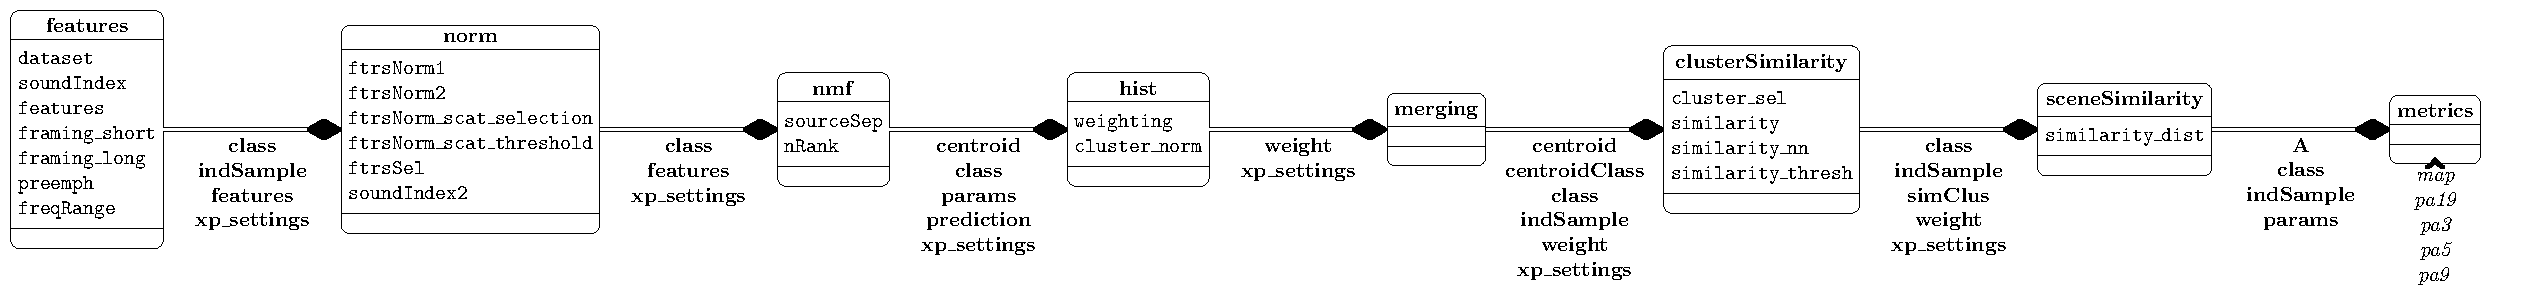
\includegraphics[width=\textwidth,height=0.8\textheight,keepaspectratio]{../figures/factors.pdf} 
  
  
\label{factorFlowGraph} 
  
  
\caption{Factors flow graph for the experiment.} 
  
  
\end{figure} 
  
  
\end{center} 
  
  
\begin{table} 
\begin{center} 
\scriptsize 
 \setlength{\tabcolsep}{.16667em} 
\begin{tabular}{lllcccc} 
nRank & similarity\_nn & similarity\_thresh & map & pa3 & pa5 & pa9 \\ 
\hline 
 5 & 0.10 & 0.05 & 0.37 & 0.55 & 0.43 & 0.33 \\ 
 5 & 0.10 & 0.10 & 0.38 & 0.56 & 0.43 & 0.32 \\ 
 5 & 0.10 & 1.00 & 0.42 & 0.60 & 0.48 & 0.38 \\ 
 5 & 0.50 & 0.05 & 0.33 & 0.51 & 0.37 & 0.29 \\ 
 5 & 0.50 & 0.10 & 0.35 & 0.54 & 0.39 & 0.29 \\ 
 5 & 0.50 & 1.00 & 0.41 & 0.59 & 0.47 & 0.36 \\ 
 5 & 1.00 & 0.05 & 0.34 & 0.50 & 0.39 & 0.29 \\ 
 5 & 1.00 & 0.10 & 0.33 & 0.49 & 0.38 & 0.30 \\ 
 5 & 1.00 & 1.00 & 0.39 & 0.60 & 0.45 & 0.35 \\ 
10 & 0.10 & 0.05 & 0.40 & 0.61 & 0.47 & 0.35 \\ 
10 & 0.10 & 0.10 & 0.41 & 0.61 & 0.49 & 0.35 \\ 
10 & 0.10 & 1.00 & 0.43 & 0.64 & 0.52 & 0.38 \\ 
10 & 0.50 & 0.05 & 0.38 & 0.58 & 0.45 & 0.32 \\ 
10 & 0.50 & 0.10 & 0.38 & 0.57 & 0.44 & 0.34 \\ 
10 & 0.50 & 1.00 & 0.42 & 0.64 & 0.51 & 0.37 \\ 
10 & 1.00 & 0.05 & 0.38 & 0.56 & 0.44 & 0.33 \\ 
10 & 1.00 & 0.10 & 0.36 & 0.50 & 0.40 & 0.32 \\ 
10 & 1.00 & 1.00 & 0.39 & 0.60 & 0.47 & 0.36 \\ 
15 & 0.10 & 0.05 & 0.40 & 0.55 & 0.45 & 0.35 \\ 
15 & 0.10 & 0.10 & 0.41 & 0.61 & 0.48 & 0.36 \\ 
15 & 0.10 & 1.00 & \textbf{\textcolor{red}{0.43}} & 0.64 & \textbf{\textcolor{red}{0.53}} & \textbf{\textcolor{red}{0.38}} \\ 
15 & 0.50 & 0.05 & 0.38 & 0.56 & 0.42 & 0.32 \\ 
15 & 0.50 & 0.10 & 0.39 & 0.56 & 0.47 & 0.35 \\ 
15 & 0.50 & 1.00 & 0.43 & \textbf{\textcolor{red}{0.65}} & 0.51 & 0.38 \\ 
15 & 1.00 & 0.05 & 0.38 & 0.55 & 0.42 & 0.33 \\ 
15 & 1.00 & 0.10 & 0.36 & 0.49 & 0.39 & 0.31 \\ 
15 & 1.00 & 1.00 & 0.39 & 0.60 & 0.47 & 0.35 \\ 
20 & 0.10 & 0.05 & 0.39 & 0.56 & 0.43 & 0.34 \\ 
20 & 0.10 & 0.10 & 0.41 & 0.61 & 0.47 & 0.36 \\ 
20 & 0.10 & 1.00 & 0.42 & 0.64 & 0.50 & 0.37 \\ 
20 & 0.50 & 0.05 & 0.39 & 0.57 & 0.46 & 0.36 \\ 
20 & 0.50 & 0.10 & 0.42 & 0.64 & 0.49 & 0.37 \\ 
20 & 0.50 & 1.00 & 0.42 & 0.64 & 0.49 & 0.37 \\ 
20 & 1.00 & 0.05 & 0.37 & 0.56 & 0.43 & 0.32 \\ 
20 & 1.00 & 0.10 & 0.39 & 0.56 & 0.46 & 0.35 \\ 
20 & 1.00 & 1.00 & 0.40 & 0.62 & 0.47 & 0.36 \\ 
\end{tabular} 
\end{center} 
\caption{dataset: train, features: scattering, framing\_long: 1\_1, preemph: 0, ftrsNorm1: null, ftrsNorm\_scat\_selection: 1, ftrsNorm\_scat\_threshold: 0.01, ftrsSel: pca\_90, sourceSep: nmf\_beta, weighting: full, cluster\_norm: null, cluster\_sel: null, similarity: gaussian\_full, similarity\_dist: emd} 
\label{datasetrFeaturscFraminlong1_1Preemp0Ftrsnorm1nuFtrsnoscatselect1Ftrsnoscatthresh0.01Ftrsselpc90SourcesepnmbeWeightfuClustenormnuClusteselnuSimilagafuSimiladistem} 
\end{table} 
 
  
\begin{table} 
\begin{center} 
\scriptsize 
 \setlength{\tabcolsep}{.16667em} 
\begin{tabular}{lllcccc} 
nRank & similarity\_nn & similarity\_thresh & map & pa3 & pa5 & pa9 \\ 
\hline 
 5 & 0.10 & 0.05 & 0.37 & 0.58 & 0.45 & 0.33 \\ 
 5 & 0.10 & 0.10 & 0.38 & 0.58 & 0.45 & 0.34 \\ 
 5 & 0.10 & 1.00 & 0.43 & 0.60 & 0.48 & 0.38 \\ 
 5 & 0.50 & 0.05 & 0.35 & 0.52 & 0.39 & 0.29 \\ 
 5 & 0.50 & 0.10 & 0.35 & 0.51 & 0.41 & 0.30 \\ 
 5 & 0.50 & 1.00 & 0.41 & 0.57 & 0.47 & 0.37 \\ 
 5 & 1.00 & 0.05 & 0.33 & 0.50 & 0.39 & 0.28 \\ 
 5 & 1.00 & 0.10 & 0.33 & 0.50 & 0.36 & 0.27 \\ 
 5 & 1.00 & 1.00 & 0.36 & 0.55 & 0.43 & 0.32 \\ 
10 & 0.10 & 0.05 & 0.38 & 0.57 & 0.44 & 0.33 \\ 
10 & 0.10 & 0.10 & 0.40 & 0.60 & 0.45 & 0.34 \\ 
10 & 0.10 & 1.00 & 0.43 & \textbf{\textcolor{red}{0.64}} & 0.49 & 0.38 \\ 
10 & 0.50 & 0.05 & 0.37 & 0.55 & 0.41 & 0.32 \\ 
10 & 0.50 & 0.10 & 0.39 & 0.57 & 0.44 & 0.34 \\ 
10 & 0.50 & 1.00 & 0.42 & 0.61 & 0.48 & 0.36 \\ 
10 & 1.00 & 0.05 & 0.34 & 0.52 & 0.41 & 0.30 \\ 
10 & 1.00 & 0.10 & 0.35 & 0.54 & 0.40 & 0.30 \\ 
10 & 1.00 & 1.00 & 0.36 & 0.55 & 0.42 & 0.31 \\ 
15 & 0.10 & 0.05 & 0.40 & 0.55 & 0.45 & 0.36 \\ 
15 & 0.10 & 0.10 & 0.43 & 0.61 & 0.49 & 0.38 \\ 
15 & 0.10 & 1.00 & \textbf{\textcolor{red}{0.44}} & 0.61 & \textbf{\textcolor{red}{0.51}} & \textbf{\textcolor{red}{0.39}} \\ 
15 & 0.50 & 0.05 & 0.39 & 0.53 & 0.43 & 0.35 \\ 
15 & 0.50 & 0.10 & 0.39 & 0.56 & 0.43 & 0.34 \\ 
15 & 0.50 & 1.00 & 0.42 & 0.59 & 0.48 & 0.37 \\ 
15 & 1.00 & 0.05 & 0.36 & 0.52 & 0.39 & 0.33 \\ 
15 & 1.00 & 0.10 & 0.35 & 0.52 & 0.39 & 0.30 \\ 
15 & 1.00 & 1.00 & 0.36 & 0.53 & 0.41 & 0.32 \\ 
20 & 0.10 & 0.05 & 0.41 & 0.60 & 0.46 & 0.36 \\ 
20 & 0.10 & 0.10 & 0.42 & 0.58 & 0.47 & 0.36 \\ 
20 & 0.10 & 1.00 & 0.43 & 0.64 & 0.50 & 0.37 \\ 
20 & 0.50 & 0.05 & 0.39 & 0.55 & 0.45 & 0.34 \\ 
20 & 0.50 & 0.10 & 0.40 & 0.57 & 0.44 & 0.35 \\ 
20 & 0.50 & 1.00 & 0.42 & 0.61 & 0.47 & 0.36 \\ 
20 & 1.00 & 0.05 & 0.36 & 0.54 & 0.41 & 0.32 \\ 
20 & 1.00 & 0.10 & 0.38 & 0.53 & 0.43 & 0.34 \\ 
20 & 1.00 & 1.00 & 0.37 & 0.55 & 0.42 & 0.32 \\ 
\end{tabular} 
\end{center} 
\caption{dataset: train, features: scattering, framing\_long: 1\_1, preemph: 0, ftrsNorm1: null, ftrsNorm\_scat\_selection: 1, ftrsNorm\_scat\_threshold: 0.01, ftrsSel: pca\_90, sourceSep: nmf\_beta, weighting: full, cluster\_norm: stand, cluster\_sel: null, similarity: gaussian\_full, similarity\_dist: emd} 
\label{datasetrFeaturscFraminlong1_1Preemp0Ftrsnorm1nuFtrsnoscatselect1Ftrsnoscatthresh0.01Ftrsselpc90SourcesepnmbeWeightfuClustenormstClusteselnuSimilagafuSimiladistem} 
\end{table} 
 
  
\begin{table} 
\begin{center} 
\scriptsize 
 \setlength{\tabcolsep}{.16667em} 
\begin{tabular}{lllcccc} 
nRank & similarity\_nn & similarity\_thresh & map & pa3 & pa5 & pa9 \\ 
\hline 
 5 & 0.10 & 0.05 & 0.35 & 0.51 & 0.39 & 0.31 \\ 
 5 & 0.10 & 0.10 & 0.36 & 0.53 & 0.41 & 0.31 \\ 
 5 & 0.10 & 1.00 & 0.41 & 0.58 & 0.45 & 0.36 \\ 
 5 & 0.50 & 0.05 & 0.33 & 0.51 & 0.38 & 0.28 \\ 
 5 & 0.50 & 0.10 & 0.35 & 0.54 & 0.41 & 0.30 \\ 
 5 & 0.50 & 1.00 & 0.40 & 0.59 & 0.46 & 0.35 \\ 
 5 & 1.00 & 0.05 & 0.33 & 0.51 & 0.36 & 0.28 \\ 
 5 & 1.00 & 0.10 & 0.34 & 0.51 & 0.39 & 0.29 \\ 
 5 & 1.00 & 1.00 & 0.40 & 0.59 & 0.45 & 0.34 \\ 
10 & 0.10 & 0.05 & 0.38 & 0.55 & 0.42 & 0.33 \\ 
10 & 0.10 & 0.10 & 0.41 & 0.59 & 0.45 & 0.35 \\ 
10 & 0.10 & 1.00 & \textbf{\textcolor{red}{0.44}} & \textbf{\textcolor{red}{0.63}} & 0.50 & 0.39 \\ 
10 & 0.50 & 0.05 & 0.39 & 0.56 & 0.44 & 0.35 \\ 
10 & 0.50 & 0.10 & 0.40 & 0.58 & 0.45 & 0.36 \\ 
10 & 0.50 & 1.00 & 0.43 & 0.62 & 0.50 & \textbf{\textcolor{red}{0.39}} \\ 
10 & 1.00 & 0.05 & 0.39 & 0.54 & 0.43 & 0.34 \\ 
10 & 1.00 & 0.10 & 0.40 & 0.57 & 0.46 & 0.36 \\ 
10 & 1.00 & 1.00 & 0.43 & 0.62 & \textbf{\textcolor{red}{0.51}} & 0.38 \\ 
15 & 0.10 & 0.05 & 0.40 & 0.57 & 0.46 & 0.35 \\ 
15 & 0.10 & 0.10 & 0.42 & 0.60 & 0.49 & 0.38 \\ 
15 & 0.10 & 1.00 & 0.43 & 0.63 & 0.51 & 0.39 \\ 
15 & 0.50 & 0.05 & 0.38 & 0.54 & 0.43 & 0.33 \\ 
15 & 0.50 & 0.10 & 0.40 & 0.59 & 0.46 & 0.35 \\ 
15 & 0.50 & 1.00 & 0.42 & 0.61 & 0.48 & 0.38 \\ 
15 & 1.00 & 0.05 & 0.39 & 0.55 & 0.44 & 0.34 \\ 
15 & 1.00 & 0.10 & 0.41 & 0.59 & 0.47 & 0.37 \\ 
15 & 1.00 & 1.00 & 0.42 & 0.61 & 0.50 & 0.37 \\ 
20 & 0.10 & 0.05 & 0.41 & 0.60 & 0.48 & 0.37 \\ 
20 & 0.10 & 0.10 & 0.43 & 0.63 & 0.49 & 0.38 \\ 
20 & 0.10 & 1.00 & 0.43 & 0.62 & 0.49 & 0.38 \\ 
20 & 0.50 & 0.05 & 0.41 & 0.57 & 0.46 & 0.37 \\ 
20 & 0.50 & 0.10 & 0.41 & 0.58 & 0.45 & 0.36 \\ 
20 & 0.50 & 1.00 & 0.42 & 0.62 & 0.48 & 0.37 \\ 
20 & 1.00 & 0.05 & 0.40 & 0.58 & 0.47 & 0.36 \\ 
20 & 1.00 & 0.10 & 0.42 & 0.61 & 0.49 & 0.37 \\ 
20 & 1.00 & 1.00 & 0.42 & 0.62 & 0.48 & 0.37 \\ 
\end{tabular} 
\end{center} 
\caption{dataset: train, features: scattering, framing\_long: 1\_1, preemph: 0, ftrsNorm1: null, ftrsNorm\_scat\_selection: 1, ftrsNorm\_scat\_threshold: 0.01, ftrsSel: pca\_90, sourceSep: nmf\_beta, weighting: full, cluster\_norm: L2, cluster\_sel: null, similarity: gaussian\_full, similarity\_dist: emd} 
\label{datasetrFeaturscFraminlong1_1Preemp0Ftrsnorm1nuFtrsnoscatselect1Ftrsnoscatthresh0.01Ftrsselpc90SourcesepnmbeWeightfuClustenormL2ClusteselnuSimilagafuSimiladistem} 
\end{table} 
 
  
\begin{table} 
\begin{center} 
\scriptsize 
 \setlength{\tabcolsep}{.16667em} 
\begin{tabular}{lllcccc} 
nRank & similarity\_nn & similarity\_thresh & map & pa3 & pa5 & pa9 \\ 
\hline 
 5 & 0.10 & 0.05 & 0.38 & 0.56 & 0.45 & 0.32 \\ 
 5 & 0.10 & 0.10 & 0.38 & 0.56 & 0.43 & 0.33 \\ 
 5 & 0.10 & 1.00 & 0.42 & 0.59 & 0.47 & 0.37 \\ 
 5 & 0.50 & 0.05 & 0.35 & 0.52 & 0.41 & 0.30 \\ 
 5 & 0.50 & 0.10 & 0.35 & 0.53 & 0.39 & 0.30 \\ 
 5 & 0.50 & 1.00 & 0.41 & 0.59 & 0.49 & 0.36 \\ 
 5 & 1.00 & 0.05 & 0.35 & 0.54 & 0.40 & 0.30 \\ 
 5 & 1.00 & 0.10 & 0.34 & 0.49 & 0.38 & 0.30 \\ 
 5 & 1.00 & 1.00 & 0.39 & 0.57 & 0.45 & 0.35 \\ 
10 & 0.10 & 0.05 & 0.40 & 0.56 & 0.45 & 0.35 \\ 
10 & 0.10 & 0.10 & 0.40 & 0.56 & 0.47 & 0.35 \\ 
10 & 0.10 & 1.00 & 0.42 & 0.58 & 0.47 & \textbf{\textcolor{red}{0.37}} \\ 
10 & 0.50 & 0.05 & 0.39 & 0.56 & 0.43 & 0.34 \\ 
10 & 0.50 & 0.10 & 0.38 & 0.54 & 0.43 & 0.33 \\ 
10 & 0.50 & 1.00 & 0.40 & 0.58 & 0.46 & 0.36 \\ 
10 & 1.00 & 0.05 & 0.38 & 0.54 & 0.44 & 0.34 \\ 
10 & 1.00 & 0.10 & 0.35 & 0.47 & 0.40 & 0.30 \\ 
10 & 1.00 & 1.00 & 0.38 & 0.56 & 0.44 & 0.34 \\ 
15 & 0.10 & 0.05 & 0.39 & 0.53 & 0.43 & 0.35 \\ 
15 & 0.10 & 0.10 & 0.40 & 0.58 & 0.43 & 0.33 \\ 
15 & 0.10 & 1.00 & \textbf{\textcolor{red}{0.42}} & 0.63 & 0.48 & 0.37 \\ 
15 & 0.50 & 0.05 & 0.37 & 0.53 & 0.42 & 0.32 \\ 
15 & 0.50 & 0.10 & 0.39 & 0.57 & 0.44 & 0.32 \\ 
15 & 0.50 & 1.00 & 0.42 & \textbf{\textcolor{red}{0.65}} & 0.47 & 0.37 \\ 
15 & 1.00 & 0.05 & 0.38 & 0.56 & 0.44 & 0.34 \\ 
15 & 1.00 & 0.10 & 0.36 & 0.51 & 0.40 & 0.30 \\ 
15 & 1.00 & 1.00 & 0.38 & 0.57 & 0.44 & 0.33 \\ 
20 & 0.10 & 0.05 & 0.38 & 0.55 & 0.43 & 0.33 \\ 
20 & 0.10 & 0.10 & 0.40 & 0.57 & 0.46 & 0.34 \\ 
20 & 0.10 & 1.00 & 0.42 & 0.62 & 0.48 & 0.37 \\ 
20 & 0.50 & 0.05 & 0.37 & 0.53 & 0.43 & 0.32 \\ 
20 & 0.50 & 0.10 & 0.40 & 0.59 & 0.46 & 0.35 \\ 
20 & 0.50 & 1.00 & 0.41 & 0.61 & \textbf{\textcolor{red}{0.49}} & 0.37 \\ 
20 & 1.00 & 0.05 & 0.36 & 0.55 & 0.42 & 0.30 \\ 
20 & 1.00 & 0.10 & 0.37 & 0.54 & 0.43 & 0.33 \\ 
20 & 1.00 & 1.00 & 0.40 & 0.60 & 0.46 & 0.35 \\ 
\end{tabular} 
\end{center} 
\caption{dataset: train, features: scattering, framing\_long: 1\_1, preemph: 0, ftrsNorm1: null, ftrsNorm\_scat\_selection: 1, ftrsNorm\_scat\_threshold: 0.01, ftrsSel: pca\_90, sourceSep: nmf\_beta, weighting: clustering, cluster\_norm: null, cluster\_sel: null, similarity: gaussian\_full, similarity\_dist: emd} 
\label{datasetrFeaturscFraminlong1_1Preemp0Ftrsnorm1nuFtrsnoscatselect1Ftrsnoscatthresh0.01Ftrsselpc90SourcesepnmbeWeightclClustenormnuClusteselnuSimilagafuSimiladistem} 
\end{table} 
 
  
\begin{table} 
\begin{center} 
\scriptsize 
 \setlength{\tabcolsep}{.16667em} 
\begin{tabular}{lllcccc} 
nRank & similarity\_nn & similarity\_thresh & map & pa3 & pa5 & pa9 \\ 
\hline 
 5 & 0.10 & 0.05 & 0.38 & 0.60 & 0.46 & 0.34 \\ 
 5 & 0.10 & 0.10 & 0.38 & 0.58 & 0.45 & 0.34 \\ 
 5 & 0.10 & 1.00 & \textbf{\textcolor{red}{0.43}} & \textbf{\textcolor{red}{0.61}} & \textbf{\textcolor{red}{0.49}} & \textbf{\textcolor{red}{0.38}} \\ 
 5 & 0.50 & 0.05 & 0.35 & 0.53 & 0.40 & 0.31 \\ 
 5 & 0.50 & 0.10 & 0.36 & 0.53 & 0.41 & 0.31 \\ 
 5 & 0.50 & 1.00 & 0.41 & 0.60 & 0.47 & 0.36 \\ 
 5 & 1.00 & 0.05 & 0.33 & 0.51 & 0.38 & 0.30 \\ 
 5 & 1.00 & 0.10 & 0.33 & 0.48 & 0.36 & 0.27 \\ 
 5 & 1.00 & 1.00 & 0.37 & 0.57 & 0.44 & 0.33 \\ 
10 & 0.10 & 0.05 & 0.37 & 0.55 & 0.40 & 0.32 \\ 
10 & 0.10 & 0.10 & 0.39 & 0.56 & 0.42 & 0.33 \\ 
10 & 0.10 & 1.00 & 0.42 & 0.58 & 0.48 & 0.37 \\ 
10 & 0.50 & 0.05 & 0.37 & 0.55 & 0.41 & 0.31 \\ 
10 & 0.50 & 0.10 & 0.39 & 0.58 & 0.44 & 0.34 \\ 
10 & 0.50 & 1.00 & 0.39 & 0.55 & 0.47 & 0.36 \\ 
10 & 1.00 & 0.05 & 0.34 & 0.52 & 0.39 & 0.28 \\ 
10 & 1.00 & 0.10 & 0.34 & 0.51 & 0.39 & 0.30 \\ 
10 & 1.00 & 1.00 & 0.35 & 0.54 & 0.41 & 0.31 \\ 
15 & 0.10 & 0.05 & 0.39 & 0.57 & 0.44 & 0.34 \\ 
15 & 0.10 & 0.10 & 0.40 & 0.57 & 0.45 & 0.35 \\ 
15 & 0.10 & 1.00 & 0.42 & 0.58 & 0.48 & 0.37 \\ 
15 & 0.50 & 0.05 & 0.37 & 0.53 & 0.42 & 0.33 \\ 
15 & 0.50 & 0.10 & 0.38 & 0.54 & 0.43 & 0.34 \\ 
15 & 0.50 & 1.00 & 0.40 & 0.55 & 0.43 & 0.35 \\ 
15 & 1.00 & 0.05 & 0.35 & 0.53 & 0.39 & 0.29 \\ 
15 & 1.00 & 0.10 & 0.35 & 0.50 & 0.39 & 0.31 \\ 
15 & 1.00 & 1.00 & 0.35 & 0.50 & 0.39 & 0.31 \\ 
20 & 0.10 & 0.05 & 0.38 & 0.56 & 0.42 & 0.33 \\ 
20 & 0.10 & 0.10 & 0.39 & 0.57 & 0.43 & 0.35 \\ 
20 & 0.10 & 1.00 & 0.42 & 0.60 & 0.47 & 0.36 \\ 
20 & 0.50 & 0.05 & 0.36 & 0.54 & 0.41 & 0.31 \\ 
20 & 0.50 & 0.10 & 0.38 & 0.56 & 0.43 & 0.33 \\ 
20 & 0.50 & 1.00 & 0.39 & 0.56 & 0.44 & 0.33 \\ 
20 & 1.00 & 0.05 & 0.33 & 0.50 & 0.36 & 0.28 \\ 
20 & 1.00 & 0.10 & 0.34 & 0.52 & 0.39 & 0.30 \\ 
20 & 1.00 & 1.00 & 0.35 & 0.50 & 0.39 & 0.30 \\ 
\end{tabular} 
\end{center} 
\caption{dataset: train, features: scattering, framing\_long: 1\_1, preemph: 0, ftrsNorm1: null, ftrsNorm\_scat\_selection: 1, ftrsNorm\_scat\_threshold: 0.01, ftrsSel: pca\_90, sourceSep: nmf\_beta, weighting: clustering, cluster\_norm: stand, cluster\_sel: null, similarity: gaussian\_full, similarity\_dist: emd} 
\label{datasetrFeaturscFraminlong1_1Preemp0Ftrsnorm1nuFtrsnoscatselect1Ftrsnoscatthresh0.01Ftrsselpc90SourcesepnmbeWeightclClustenormstClusteselnuSimilagafuSimiladistem} 
\end{table} 
 
  
\begin{table} 
\begin{center} 
\scriptsize 
 \setlength{\tabcolsep}{.16667em} 
\begin{tabular}{lllcccc} 
nRank & similarity\_nn & similarity\_thresh & map & pa3 & pa5 & pa9 \\ 
\hline 
 5 & 0.10 & 0.05 & 0.36 & 0.51 & 0.40 & 0.31 \\ 
 5 & 0.10 & 0.10 & 0.37 & 0.54 & 0.40 & 0.31 \\ 
 5 & 0.10 & 1.00 & 0.41 & 0.59 & 0.46 & 0.35 \\ 
 5 & 0.50 & 0.05 & 0.34 & 0.52 & 0.41 & 0.28 \\ 
 5 & 0.50 & 0.10 & 0.35 & 0.54 & 0.40 & 0.31 \\ 
 5 & 0.50 & 1.00 & 0.41 & 0.58 & 0.45 & 0.35 \\ 
 5 & 1.00 & 0.05 & 0.34 & 0.52 & 0.41 & 0.29 \\ 
 5 & 1.00 & 0.10 & 0.34 & 0.51 & 0.40 & 0.29 \\ 
 5 & 1.00 & 1.00 & 0.40 & 0.58 & 0.44 & 0.35 \\ 
10 & 0.10 & 0.05 & 0.38 & 0.52 & 0.41 & 0.32 \\ 
10 & 0.10 & 0.10 & 0.39 & 0.54 & 0.44 & 0.35 \\ 
10 & 0.10 & 1.00 & \textbf{\textcolor{red}{0.43}} & 0.59 & \textbf{\textcolor{red}{0.49}} & \textbf{\textcolor{red}{0.38}} \\ 
10 & 0.50 & 0.05 & 0.38 & 0.55 & 0.44 & 0.34 \\ 
10 & 0.50 & 0.10 & 0.38 & 0.52 & 0.41 & 0.33 \\ 
10 & 0.50 & 1.00 & 0.41 & 0.57 & 0.47 & 0.35 \\ 
10 & 1.00 & 0.05 & 0.38 & 0.54 & 0.41 & 0.33 \\ 
10 & 1.00 & 0.10 & 0.40 & 0.55 & 0.43 & 0.35 \\ 
10 & 1.00 & 1.00 & 0.41 & 0.58 & 0.46 & 0.36 \\ 
15 & 0.10 & 0.05 & 0.38 & 0.53 & 0.43 & 0.34 \\ 
15 & 0.10 & 0.10 & 0.39 & 0.55 & 0.43 & 0.34 \\ 
15 & 0.10 & 1.00 & 0.42 & 0.60 & 0.46 & 0.36 \\ 
15 & 0.50 & 0.05 & 0.39 & 0.54 & 0.41 & 0.34 \\ 
15 & 0.50 & 0.10 & 0.39 & 0.53 & 0.42 & 0.33 \\ 
15 & 0.50 & 1.00 & 0.40 & 0.57 & 0.44 & 0.36 \\ 
15 & 1.00 & 0.05 & 0.38 & 0.51 & 0.42 & 0.34 \\ 
15 & 1.00 & 0.10 & 0.38 & 0.53 & 0.42 & 0.33 \\ 
15 & 1.00 & 1.00 & 0.40 & 0.57 & 0.46 & 0.37 \\ 
20 & 0.10 & 0.05 & 0.40 & 0.57 & 0.46 & 0.35 \\ 
20 & 0.10 & 0.10 & 0.41 & 0.59 & 0.46 & 0.35 \\ 
20 & 0.10 & 1.00 & 0.41 & \textbf{\textcolor{red}{0.60}} & 0.46 & 0.36 \\ 
20 & 0.50 & 0.05 & 0.39 & 0.57 & 0.44 & 0.33 \\ 
20 & 0.50 & 0.10 & 0.40 & 0.60 & 0.44 & 0.34 \\ 
20 & 0.50 & 1.00 & 0.40 & 0.59 & 0.46 & 0.35 \\ 
20 & 1.00 & 0.05 & 0.38 & 0.56 & 0.44 & 0.33 \\ 
20 & 1.00 & 0.10 & 0.39 & 0.58 & 0.44 & 0.34 \\ 
20 & 1.00 & 1.00 & 0.40 & 0.58 & 0.46 & 0.34 \\ 
\end{tabular} 
\end{center} 
\caption{dataset: train, features: scattering, framing\_long: 1\_1, preemph: 0, ftrsNorm1: null, ftrsNorm\_scat\_selection: 1, ftrsNorm\_scat\_threshold: 0.01, ftrsSel: pca\_90, sourceSep: nmf\_beta, weighting: clustering, cluster\_norm: L2, cluster\_sel: null, similarity: gaussian\_full, similarity\_dist: emd} 
\label{datasetrFeaturscFraminlong1_1Preemp0Ftrsnorm1nuFtrsnoscatselect1Ftrsnoscatthresh0.01Ftrsselpc90SourcesepnmbeWeightclClustenormL2ClusteselnuSimilagafuSimiladistem} 
\end{table} 
 
  
\begin{table} 
\begin{center} 
\scriptsize 
 \setlength{\tabcolsep}{.16667em} 
\begin{tabular}{lllcccc} 
nRank & similarity\_nn & similarity\_thresh & map & pa3 & pa5 & pa9 \\ 
\hline 
 5 & 0.10 & 0.05 & 0.35 & 0.53 & 0.37 & 0.30 \\ 
 5 & 0.10 & 0.10 & 0.36 & 0.51 & 0.40 & 0.30 \\ 
 5 & 0.10 & 1.00 & 0.40 & 0.57 & 0.45 & 0.35 \\ 
 5 & 0.50 & 0.05 & 0.34 & 0.51 & 0.38 & 0.29 \\ 
 5 & 0.50 & 0.10 & 0.34 & 0.53 & 0.41 & 0.29 \\ 
 5 & 0.50 & 1.00 & 0.40 & 0.56 & 0.46 & 0.36 \\ 
 5 & 1.00 & 0.05 & 0.34 & 0.50 & 0.38 & 0.28 \\ 
 5 & 1.00 & 0.10 & 0.33 & 0.47 & 0.37 & 0.28 \\ 
 5 & 1.00 & 1.00 & 0.39 & 0.58 & 0.45 & 0.35 \\ 
10 & 0.10 & 0.05 & 0.39 & 0.58 & 0.45 & 0.34 \\ 
10 & 0.10 & 0.10 & 0.40 & 0.59 & 0.46 & 0.33 \\ 
10 & 0.10 & 1.00 & 0.42 & 0.62 & 0.49 & 0.37 \\ 
10 & 0.50 & 0.05 & 0.36 & 0.55 & 0.45 & 0.32 \\ 
10 & 0.50 & 0.10 & 0.37 & 0.55 & 0.43 & 0.31 \\ 
10 & 0.50 & 1.00 & 0.41 & 0.61 & 0.48 & 0.37 \\ 
10 & 1.00 & 0.05 & 0.36 & 0.54 & 0.40 & 0.31 \\ 
10 & 1.00 & 0.10 & 0.37 & 0.57 & 0.43 & 0.32 \\ 
10 & 1.00 & 1.00 & 0.39 & 0.60 & 0.47 & 0.35 \\ 
15 & 0.10 & 0.05 & 0.41 & 0.59 & 0.47 & 0.35 \\ 
15 & 0.10 & 0.10 & 0.41 & 0.61 & 0.48 & 0.36 \\ 
15 & 0.10 & 1.00 & \textbf{\textcolor{red}{0.43}} & 0.62 & \textbf{\textcolor{red}{0.52}} & \textbf{\textcolor{red}{0.38}} \\ 
15 & 0.50 & 0.05 & 0.40 & 0.59 & 0.46 & 0.35 \\ 
15 & 0.50 & 0.10 & 0.39 & 0.56 & 0.44 & 0.35 \\ 
15 & 0.50 & 1.00 & 0.42 & \textbf{\textcolor{red}{0.63}} & 0.50 & 0.37 \\ 
15 & 1.00 & 0.05 & 0.39 & 0.55 & 0.45 & 0.34 \\ 
15 & 1.00 & 0.10 & 0.38 & 0.53 & 0.42 & 0.34 \\ 
15 & 1.00 & 1.00 & 0.39 & 0.61 & 0.48 & 0.35 \\ 
20 & 0.10 & 0.05 & 0.40 & 0.58 & 0.46 & 0.37 \\ 
20 & 0.10 & 0.10 & 0.41 & 0.56 & 0.47 & 0.37 \\ 
20 & 0.10 & 1.00 & 0.42 & 0.63 & 0.49 & \textbf{\textcolor{red}{0.38}} \\ 
20 & 0.50 & 0.05 & 0.39 & 0.58 & 0.46 & 0.34 \\ 
20 & 0.50 & 0.10 & 0.40 & 0.60 & 0.47 & 0.35 \\ 
20 & 0.50 & 1.00 & 0.42 & 0.62 & 0.49 & 0.37 \\ 
20 & 1.00 & 0.05 & 0.37 & 0.56 & 0.42 & 0.32 \\ 
20 & 1.00 & 0.10 & 0.40 & 0.57 & 0.45 & 0.36 \\ 
20 & 1.00 & 1.00 & 0.40 & 0.62 & 0.48 & 0.36 \\ 
\end{tabular} 
\end{center} 
\caption{dataset: train, features: scattering, framing\_long: 1\_1, preemph: 0, ftrsNorm1: null, ftrsNorm\_scat\_selection: 1, ftrsNorm\_scat\_threshold: 0.01, ftrsSel: pca\_90, sourceSep: nmf\_beta, weighting: full, cluster\_norm: null, cluster\_sel: pca\_90, similarity: gaussian\_full, similarity\_dist: emd} 
\label{datasetrFeaturscFraminlong1_1Preemp0Ftrsnorm1nuFtrsnoscatselect1Ftrsnoscatthresh0.01Ftrsselpc90SourcesepnmbeWeightfuClustenormnuClusteselpc90SimilagafuSimiladistem} 
\end{table} 
 
  
\begin{table} 
\begin{center} 
\scriptsize 
 \setlength{\tabcolsep}{.16667em} 
\begin{tabular}{lllcccc} 
nRank & similarity\_nn & similarity\_thresh & map & pa3 & pa5 & pa9 \\ 
\hline 
 5 & 0.10 & 0.05 & 0.39 & 0.57 & 0.46 & 0.35 \\ 
 5 & 0.10 & 0.10 & 0.39 & 0.57 & 0.44 & 0.33 \\ 
 5 & 0.10 & 1.00 & \textbf{\textcolor{red}{0.44}} & 0.61 & 0.50 & 0.39 \\ 
 5 & 0.50 & 0.05 & 0.35 & 0.53 & 0.42 & 0.31 \\ 
 5 & 0.50 & 0.10 & 0.37 & 0.55 & 0.44 & 0.33 \\ 
 5 & 0.50 & 1.00 & 0.42 & 0.61 & 0.48 & 0.38 \\ 
 5 & 1.00 & 0.05 & 0.35 & 0.53 & 0.39 & 0.30 \\ 
 5 & 1.00 & 0.10 & 0.35 & 0.50 & 0.40 & 0.31 \\ 
 5 & 1.00 & 1.00 & 0.37 & 0.56 & 0.43 & 0.33 \\ 
10 & 0.10 & 0.05 & 0.38 & 0.59 & 0.44 & 0.33 \\ 
10 & 0.10 & 0.10 & 0.40 & 0.59 & 0.46 & 0.35 \\ 
10 & 0.10 & 1.00 & 0.43 & 0.63 & 0.49 & 0.36 \\ 
10 & 0.50 & 0.05 & 0.37 & 0.56 & 0.43 & 0.33 \\ 
10 & 0.50 & 0.10 & 0.37 & 0.55 & 0.43 & 0.32 \\ 
10 & 0.50 & 1.00 & 0.41 & 0.61 & 0.48 & 0.37 \\ 
10 & 1.00 & 0.05 & 0.33 & 0.48 & 0.36 & 0.28 \\ 
10 & 1.00 & 0.10 & 0.33 & 0.49 & 0.37 & 0.27 \\ 
10 & 1.00 & 1.00 & 0.35 & 0.55 & 0.41 & 0.31 \\ 
15 & 0.10 & 0.05 & 0.40 & 0.59 & 0.44 & 0.35 \\ 
15 & 0.10 & 0.10 & 0.41 & 0.58 & 0.47 & 0.36 \\ 
15 & 0.10 & 1.00 & 0.43 & 0.61 & 0.50 & \textbf{\textcolor{red}{0.40}} \\ 
15 & 0.50 & 0.05 & 0.39 & 0.56 & 0.45 & 0.34 \\ 
15 & 0.50 & 0.10 & 0.38 & 0.53 & 0.43 & 0.33 \\ 
15 & 0.50 & 1.00 & 0.41 & 0.59 & 0.48 & 0.37 \\ 
15 & 1.00 & 0.05 & 0.35 & 0.52 & 0.40 & 0.31 \\ 
15 & 1.00 & 0.10 & 0.34 & 0.48 & 0.38 & 0.30 \\ 
15 & 1.00 & 1.00 & 0.35 & 0.51 & 0.40 & 0.31 \\ 
20 & 0.10 & 0.05 & 0.39 & 0.57 & 0.44 & 0.35 \\ 
20 & 0.10 & 0.10 & 0.42 & 0.58 & 0.46 & 0.37 \\ 
20 & 0.10 & 1.00 & 0.43 & \textbf{\textcolor{red}{0.64}} & \textbf{\textcolor{red}{0.50}} & 0.37 \\ 
20 & 0.50 & 0.05 & 0.38 & 0.53 & 0.43 & 0.33 \\ 
20 & 0.50 & 0.10 & 0.40 & 0.58 & 0.46 & 0.35 \\ 
20 & 0.50 & 1.00 & 0.42 & 0.61 & 0.48 & 0.37 \\ 
20 & 1.00 & 0.05 & 0.37 & 0.53 & 0.42 & 0.33 \\ 
20 & 1.00 & 0.10 & 0.36 & 0.53 & 0.40 & 0.31 \\ 
20 & 1.00 & 1.00 & 0.37 & 0.53 & 0.41 & 0.32 \\ 
\end{tabular} 
\end{center} 
\caption{dataset: train, features: scattering, framing\_long: 1\_1, preemph: 0, ftrsNorm1: null, ftrsNorm\_scat\_selection: 1, ftrsNorm\_scat\_threshold: 0.01, ftrsSel: pca\_90, sourceSep: nmf\_beta, weighting: full, cluster\_norm: stand, cluster\_sel: pca\_90, similarity: gaussian\_full, similarity\_dist: emd} 
\label{datasetrFeaturscFraminlong1_1Preemp0Ftrsnorm1nuFtrsnoscatselect1Ftrsnoscatthresh0.01Ftrsselpc90SourcesepnmbeWeightfuClustenormstClusteselpc90SimilagafuSimiladistem} 
\end{table} 
 
  
\begin{table} 
\begin{center} 
\scriptsize 
 \setlength{\tabcolsep}{.16667em} 
\begin{tabular}{lllcccc} 
nRank & similarity\_nn & similarity\_thresh & map & pa3 & pa5 & pa9 \\ 
\hline 
 5 & 0.10 & 0.05 & 0.35 & 0.50 & 0.37 & 0.29 \\ 
 5 & 0.10 & 0.10 & 0.36 & 0.53 & 0.40 & 0.31 \\ 
 5 & 0.10 & 1.00 & 0.40 & 0.59 & 0.45 & 0.35 \\ 
 5 & 0.50 & 0.05 & 0.32 & 0.51 & 0.36 & 0.28 \\ 
 5 & 0.50 & 0.10 & 0.34 & 0.52 & 0.41 & 0.29 \\ 
 5 & 0.50 & 1.00 & 0.40 & 0.60 & 0.45 & 0.34 \\ 
 5 & 1.00 & 0.05 & 0.32 & 0.48 & 0.34 & 0.28 \\ 
 5 & 1.00 & 0.10 & 0.34 & 0.51 & 0.40 & 0.28 \\ 
 5 & 1.00 & 1.00 & 0.40 & 0.60 & 0.47 & 0.34 \\ 
10 & 0.10 & 0.05 & 0.40 & 0.57 & 0.47 & 0.36 \\ 
10 & 0.10 & 0.10 & 0.41 & 0.59 & 0.47 & 0.36 \\ 
10 & 0.10 & 1.00 & \textbf{\textcolor{red}{0.44}} & 0.62 & \textbf{\textcolor{red}{0.51}} & \textbf{\textcolor{red}{0.40}} \\ 
10 & 0.50 & 0.05 & 0.38 & 0.54 & 0.43 & 0.33 \\ 
10 & 0.50 & 0.10 & 0.40 & 0.56 & 0.46 & 0.37 \\ 
10 & 0.50 & 1.00 & 0.43 & 0.61 & 0.50 & 0.38 \\ 
10 & 1.00 & 0.05 & 0.38 & 0.55 & 0.43 & 0.32 \\ 
10 & 1.00 & 0.10 & 0.40 & 0.57 & 0.46 & 0.35 \\ 
10 & 1.00 & 1.00 & 0.43 & 0.61 & 0.50 & 0.39 \\ 
15 & 0.10 & 0.05 & 0.39 & 0.56 & 0.47 & 0.35 \\ 
15 & 0.10 & 0.10 & 0.41 & 0.60 & 0.48 & 0.37 \\ 
15 & 0.10 & 1.00 & 0.43 & 0.62 & 0.51 & 0.38 \\ 
15 & 0.50 & 0.05 & 0.38 & 0.53 & 0.43 & 0.34 \\ 
15 & 0.50 & 0.10 & 0.40 & 0.56 & 0.46 & 0.37 \\ 
15 & 0.50 & 1.00 & 0.42 & 0.62 & 0.49 & 0.38 \\ 
15 & 1.00 & 0.05 & 0.37 & 0.50 & 0.41 & 0.32 \\ 
15 & 1.00 & 0.10 & 0.38 & 0.55 & 0.43 & 0.33 \\ 
15 & 1.00 & 1.00 & 0.42 & 0.62 & 0.49 & 0.37 \\ 
20 & 0.10 & 0.05 & 0.43 & \textbf{\textcolor{red}{0.63}} & 0.50 & 0.39 \\ 
20 & 0.10 & 0.10 & 0.44 & 0.63 & 0.50 & 0.39 \\ 
20 & 0.10 & 1.00 & 0.43 & 0.62 & 0.50 & 0.38 \\ 
20 & 0.50 & 0.05 & 0.40 & 0.60 & 0.47 & 0.35 \\ 
20 & 0.50 & 0.10 & 0.41 & 0.57 & 0.47 & 0.38 \\ 
20 & 0.50 & 1.00 & 0.42 & 0.63 & 0.49 & 0.37 \\ 
20 & 1.00 & 0.05 & 0.41 & 0.58 & 0.46 & 0.37 \\ 
20 & 1.00 & 0.10 & 0.42 & 0.60 & 0.48 & 0.36 \\ 
20 & 1.00 & 1.00 & 0.42 & 0.63 & 0.49 & 0.37 \\ 
\end{tabular} 
\end{center} 
\caption{dataset: train, features: scattering, framing\_long: 1\_1, preemph: 0, ftrsNorm1: null, ftrsNorm\_scat\_selection: 1, ftrsNorm\_scat\_threshold: 0.01, ftrsSel: pca\_90, sourceSep: nmf\_beta, weighting: full, cluster\_norm: L2, cluster\_sel: pca\_90, similarity: gaussian\_full, similarity\_dist: emd} 
\label{datasetrFeaturscFraminlong1_1Preemp0Ftrsnorm1nuFtrsnoscatselect1Ftrsnoscatthresh0.01Ftrsselpc90SourcesepnmbeWeightfuClustenormL2Clusteselpc90SimilagafuSimiladistem} 
\end{table} 
 
  
\begin{table} 
\begin{center} 
\scriptsize 
 \setlength{\tabcolsep}{.16667em} 
\begin{tabular}{lllcccc} 
nRank & similarity\_nn & similarity\_thresh & map & pa3 & pa5 & pa9 \\ 
\hline 
 5 & 0.10 & 0.05 & 0.36 & 0.50 & 0.39 & 0.31 \\ 
 5 & 0.10 & 0.10 & 0.36 & 0.51 & 0.39 & 0.30 \\ 
 5 & 0.10 & 1.00 & 0.41 & 0.58 & 0.46 & 0.35 \\ 
 5 & 0.50 & 0.05 & 0.36 & 0.54 & 0.41 & 0.32 \\ 
 5 & 0.50 & 0.10 & 0.35 & 0.54 & 0.40 & 0.29 \\ 
 5 & 0.50 & 1.00 & 0.41 & 0.58 & 0.48 & 0.36 \\ 
 5 & 1.00 & 0.05 & 0.35 & 0.51 & 0.38 & 0.29 \\ 
 5 & 1.00 & 0.10 & 0.34 & 0.47 & 0.38 & 0.28 \\ 
 5 & 1.00 & 1.00 & 0.39 & 0.57 & 0.44 & 0.34 \\ 
10 & 0.10 & 0.05 & 0.39 & 0.55 & 0.44 & 0.34 \\ 
10 & 0.10 & 0.10 & 0.40 & 0.57 & 0.44 & 0.34 \\ 
10 & 0.10 & 1.00 & 0.41 & 0.58 & 0.46 & 0.36 \\ 
10 & 0.50 & 0.05 & 0.36 & 0.53 & 0.43 & 0.32 \\ 
10 & 0.50 & 0.10 & 0.36 & 0.50 & 0.40 & 0.31 \\ 
10 & 0.50 & 1.00 & 0.40 & 0.57 & 0.45 & 0.35 \\ 
10 & 1.00 & 0.05 & 0.35 & 0.53 & 0.40 & 0.31 \\ 
10 & 1.00 & 0.10 & 0.37 & 0.54 & 0.42 & 0.32 \\ 
10 & 1.00 & 1.00 & 0.38 & 0.56 & 0.44 & 0.34 \\ 
15 & 0.10 & 0.05 & 0.40 & 0.56 & 0.43 & 0.35 \\ 
15 & 0.10 & 0.10 & 0.40 & 0.56 & 0.43 & 0.35 \\ 
15 & 0.10 & 1.00 & \textbf{\textcolor{red}{0.42}} & 0.60 & 0.47 & 0.37 \\ 
15 & 0.50 & 0.05 & 0.38 & 0.55 & 0.41 & 0.32 \\ 
15 & 0.50 & 0.10 & 0.38 & 0.56 & 0.43 & 0.33 \\ 
15 & 0.50 & 1.00 & 0.41 & 0.59 & 0.47 & 0.36 \\ 
15 & 1.00 & 0.05 & 0.38 & 0.55 & 0.43 & 0.33 \\ 
15 & 1.00 & 0.10 & 0.37 & 0.51 & 0.41 & 0.32 \\ 
15 & 1.00 & 1.00 & 0.38 & 0.56 & 0.44 & 0.34 \\ 
20 & 0.10 & 0.05 & 0.39 & 0.58 & 0.44 & 0.35 \\ 
20 & 0.10 & 0.10 & 0.41 & 0.59 & 0.49 & 0.37 \\ 
20 & 0.10 & 1.00 & 0.42 & \textbf{\textcolor{red}{0.61}} & 0.48 & 0.36 \\ 
20 & 0.50 & 0.05 & 0.38 & 0.58 & 0.45 & 0.34 \\ 
20 & 0.50 & 0.10 & 0.39 & 0.58 & 0.47 & 0.34 \\ 
20 & 0.50 & 1.00 & 0.41 & 0.60 & \textbf{\textcolor{red}{0.49}} & \textbf{\textcolor{red}{0.37}} \\ 
20 & 1.00 & 0.05 & 0.36 & 0.53 & 0.42 & 0.31 \\ 
20 & 1.00 & 0.10 & 0.38 & 0.54 & 0.43 & 0.33 \\ 
20 & 1.00 & 1.00 & 0.40 & 0.57 & 0.47 & 0.35 \\ 
\end{tabular} 
\end{center} 
\caption{dataset: train, features: scattering, framing\_long: 1\_1, preemph: 0, ftrsNorm1: null, ftrsNorm\_scat\_selection: 1, ftrsNorm\_scat\_threshold: 0.01, ftrsSel: pca\_90, sourceSep: nmf\_beta, weighting: clustering, cluster\_norm: null, cluster\_sel: pca\_90, similarity: gaussian\_full, similarity\_dist: emd} 
\label{datasetrFeaturscFraminlong1_1Preemp0Ftrsnorm1nuFtrsnoscatselect1Ftrsnoscatthresh0.01Ftrsselpc90SourcesepnmbeWeightclClustenormnuClusteselpc90SimilagafuSimiladistem} 
\end{table} 
 
  
\clearpage 
  
  
\begin{table} 
\begin{center} 
\scriptsize 
 \setlength{\tabcolsep}{.16667em} 
\begin{tabular}{lllcccc} 
nRank & similarity\_nn & similarity\_thresh & map & pa3 & pa5 & pa9 \\ 
\hline 
 5 & 0.10 & 0.05 & 0.39 & 0.57 & 0.47 & 0.34 \\ 
 5 & 0.10 & 0.10 & 0.39 & 0.55 & 0.44 & 0.34 \\ 
 5 & 0.10 & 1.00 & \textbf{\textcolor{red}{0.44}} & \textbf{\textcolor{red}{0.61}} & \textbf{\textcolor{red}{0.51}} & \textbf{\textcolor{red}{0.39}} \\ 
 5 & 0.50 & 0.05 & 0.35 & 0.55 & 0.41 & 0.31 \\ 
 5 & 0.50 & 0.10 & 0.37 & 0.55 & 0.45 & 0.34 \\ 
 5 & 0.50 & 1.00 & 0.42 & 0.60 & 0.49 & 0.38 \\ 
 5 & 1.00 & 0.05 & 0.35 & 0.52 & 0.40 & 0.29 \\ 
 5 & 1.00 & 0.10 & 0.35 & 0.52 & 0.40 & 0.30 \\ 
 5 & 1.00 & 1.00 & 0.37 & 0.54 & 0.42 & 0.34 \\ 
10 & 0.10 & 0.05 & 0.37 & 0.56 & 0.44 & 0.34 \\ 
10 & 0.10 & 0.10 & 0.38 & 0.58 & 0.45 & 0.34 \\ 
10 & 0.10 & 1.00 & 0.41 & 0.59 & 0.49 & 0.36 \\ 
10 & 0.50 & 0.05 & 0.36 & 0.52 & 0.42 & 0.33 \\ 
10 & 0.50 & 0.10 & 0.36 & 0.54 & 0.42 & 0.32 \\ 
10 & 0.50 & 1.00 & 0.39 & 0.55 & 0.46 & 0.35 \\ 
10 & 1.00 & 0.05 & 0.32 & 0.47 & 0.36 & 0.27 \\ 
10 & 1.00 & 0.10 & 0.31 & 0.46 & 0.34 & 0.26 \\ 
10 & 1.00 & 1.00 & 0.34 & 0.52 & 0.40 & 0.31 \\ 
15 & 0.10 & 0.05 & 0.38 & 0.55 & 0.43 & 0.33 \\ 
15 & 0.10 & 0.10 & 0.39 & 0.54 & 0.46 & 0.35 \\ 
15 & 0.10 & 1.00 & 0.41 & 0.58 & 0.47 & 0.36 \\ 
15 & 0.50 & 0.05 & 0.37 & 0.55 & 0.42 & 0.32 \\ 
15 & 0.50 & 0.10 & 0.36 & 0.53 & 0.39 & 0.30 \\ 
15 & 0.50 & 1.00 & 0.39 & 0.56 & 0.43 & 0.34 \\ 
15 & 1.00 & 0.05 & 0.35 & 0.51 & 0.40 & 0.30 \\ 
15 & 1.00 & 0.10 & 0.32 & 0.47 & 0.36 & 0.28 \\ 
15 & 1.00 & 1.00 & 0.34 & 0.49 & 0.37 & 0.30 \\ 
20 & 0.10 & 0.05 & 0.37 & 0.56 & 0.42 & 0.31 \\ 
20 & 0.10 & 0.10 & 0.39 & 0.55 & 0.43 & 0.33 \\ 
20 & 0.10 & 1.00 & 0.41 & 0.58 & 0.46 & 0.37 \\ 
20 & 0.50 & 0.05 & 0.36 & 0.52 & 0.39 & 0.31 \\ 
20 & 0.50 & 0.10 & 0.38 & 0.57 & 0.43 & 0.34 \\ 
20 & 0.50 & 1.00 & 0.38 & 0.55 & 0.45 & 0.33 \\ 
20 & 1.00 & 0.05 & 0.33 & 0.49 & 0.38 & 0.29 \\ 
20 & 1.00 & 0.10 & 0.34 & 0.50 & 0.39 & 0.29 \\ 
20 & 1.00 & 1.00 & 0.34 & 0.49 & 0.38 & 0.29 \\ 
\end{tabular} 
\end{center} 
\caption{dataset: train, features: scattering, framing\_long: 1\_1, preemph: 0, ftrsNorm1: null, ftrsNorm\_scat\_selection: 1, ftrsNorm\_scat\_threshold: 0.01, ftrsSel: pca\_90, sourceSep: nmf\_beta, weighting: clustering, cluster\_norm: stand, cluster\_sel: pca\_90, similarity: gaussian\_full, similarity\_dist: emd} 
\label{datasetrFeaturscFraminlong1_1Preemp0Ftrsnorm1nuFtrsnoscatselect1Ftrsnoscatthresh0.01Ftrsselpc90SourcesepnmbeWeightclClustenormstClusteselpc90SimilagafuSimiladistem} 
\end{table} 
 
  
\begin{table} 
\begin{center} 
\scriptsize 
 \setlength{\tabcolsep}{.16667em} 
\begin{tabular}{lllcccc} 
nRank & similarity\_nn & similarity\_thresh & map & pa3 & pa5 & pa9 \\ 
\hline 
 5 & 0.10 & 0.05 & 0.36 & 0.52 & 0.40 & 0.31 \\ 
 5 & 0.10 & 0.10 & 0.36 & 0.52 & 0.40 & 0.31 \\ 
 5 & 0.10 & 1.00 & 0.40 & 0.58 & 0.46 & 0.34 \\ 
 5 & 0.50 & 0.05 & 0.33 & 0.50 & 0.38 & 0.29 \\ 
 5 & 0.50 & 0.10 & 0.34 & 0.51 & 0.39 & 0.30 \\ 
 5 & 0.50 & 1.00 & 0.40 & 0.59 & 0.46 & 0.35 \\ 
 5 & 1.00 & 0.05 & 0.33 & 0.48 & 0.38 & 0.30 \\ 
 5 & 1.00 & 0.10 & 0.34 & 0.54 & 0.40 & 0.28 \\ 
 5 & 1.00 & 1.00 & 0.40 & 0.57 & 0.46 & 0.35 \\ 
10 & 0.10 & 0.05 & 0.39 & 0.56 & 0.45 & 0.35 \\ 
10 & 0.10 & 0.10 & 0.39 & 0.54 & 0.43 & 0.35 \\ 
10 & 0.10 & 1.00 & \textbf{\textcolor{red}{0.43}} & 0.57 & \textbf{\textcolor{red}{0.48}} & \textbf{\textcolor{red}{0.38}} \\ 
10 & 0.50 & 0.05 & 0.37 & 0.51 & 0.42 & 0.32 \\ 
10 & 0.50 & 0.10 & 0.38 & 0.53 & 0.42 & 0.34 \\ 
10 & 0.50 & 1.00 & 0.41 & 0.58 & 0.46 & 0.35 \\ 
10 & 1.00 & 0.05 & 0.37 & 0.52 & 0.40 & 0.31 \\ 
10 & 1.00 & 0.10 & 0.37 & 0.51 & 0.41 & 0.32 \\ 
10 & 1.00 & 1.00 & 0.41 & 0.57 & 0.46 & 0.35 \\ 
15 & 0.10 & 0.05 & 0.38 & 0.54 & 0.42 & 0.34 \\ 
15 & 0.10 & 0.10 & 0.39 & 0.56 & 0.44 & 0.35 \\ 
15 & 0.10 & 1.00 & 0.41 & 0.59 & 0.46 & 0.36 \\ 
15 & 0.50 & 0.05 & 0.37 & 0.51 & 0.41 & 0.33 \\ 
15 & 0.50 & 0.10 & 0.38 & 0.55 & 0.42 & 0.33 \\ 
15 & 0.50 & 1.00 & 0.40 & 0.56 & 0.46 & 0.36 \\ 
15 & 1.00 & 0.05 & 0.37 & 0.48 & 0.37 & 0.33 \\ 
15 & 1.00 & 0.10 & 0.38 & 0.54 & 0.43 & 0.32 \\ 
15 & 1.00 & 1.00 & 0.40 & 0.56 & 0.45 & 0.36 \\ 
20 & 0.10 & 0.05 & 0.39 & 0.55 & 0.45 & 0.35 \\ 
20 & 0.10 & 0.10 & 0.41 & 0.59 & 0.47 & 0.36 \\ 
20 & 0.10 & 1.00 & 0.42 & 0.60 & 0.47 & 0.36 \\ 
20 & 0.50 & 0.05 & 0.38 & 0.57 & 0.44 & 0.32 \\ 
20 & 0.50 & 0.10 & 0.39 & 0.56 & 0.43 & 0.33 \\ 
20 & 0.50 & 1.00 & 0.40 & \textbf{\textcolor{red}{0.60}} & 0.46 & 0.35 \\ 
20 & 1.00 & 0.05 & 0.38 & 0.55 & 0.44 & 0.33 \\ 
20 & 1.00 & 0.10 & 0.39 & 0.55 & 0.43 & 0.33 \\ 
20 & 1.00 & 1.00 & 0.40 & 0.58 & 0.46 & 0.34 \\ 
\end{tabular} 
\end{center} 
\caption{dataset: train, features: scattering, framing\_long: 1\_1, preemph: 0, ftrsNorm1: null, ftrsNorm\_scat\_selection: 1, ftrsNorm\_scat\_threshold: 0.01, ftrsSel: pca\_90, sourceSep: nmf\_beta, weighting: clustering, cluster\_norm: L2, cluster\_sel: pca\_90, similarity: gaussian\_full, similarity\_dist: emd} 
\label{datasetrFeaturscFraminlong1_1Preemp0Ftrsnorm1nuFtrsnoscatselect1Ftrsnoscatthresh0.01Ftrsselpc90SourcesepnmbeWeightclClustenormL2Clusteselpc90SimilagafuSimiladistem} 
\end{table} 
 
  
\begin{table} 
\begin{center} 
\scriptsize 
 \setlength{\tabcolsep}{.16667em} 
\begin{tabular}{lllcccc} 
nRank & similarity\_nn & similarity\_thresh & map & pa3 & pa5 & pa9 \\ 
\hline 
 5 & 0.10 & 0.05 & 0.41 & 0.61 & 0.49 & 0.37 \\ 
 5 & 0.10 & 0.10 & 0.40 & 0.60 & 0.47 & 0.36 \\ 
 5 & 0.10 & 1.00 & 0.47 & 0.65 & 0.52 & 0.42 \\ 
 5 & 0.50 & 0.05 & 0.40 & 0.57 & 0.46 & 0.35 \\ 
 5 & 0.50 & 0.10 & 0.40 & 0.58 & 0.47 & 0.35 \\ 
 5 & 0.50 & 1.00 & 0.47 & \textbf{\textcolor{red}{0.65}} & 0.51 & 0.40 \\ 
 5 & 1.00 & 0.05 & 0.35 & 0.52 & 0.39 & 0.31 \\ 
 5 & 1.00 & 0.10 & 0.36 & 0.53 & 0.41 & 0.31 \\ 
 5 & 1.00 & 1.00 & 0.43 & 0.58 & 0.46 & 0.37 \\ 
10 & 0.10 & 0.05 & 0.45 & 0.59 & 0.47 & 0.40 \\ 
10 & 0.10 & 0.10 & 0.47 & 0.62 & \textbf{\textcolor{red}{0.54}} & 0.42 \\ 
10 & 0.10 & 1.00 & \textbf{\textcolor{red}{0.49}} & 0.64 & 0.52 & \textbf{\textcolor{red}{0.43}} \\ 
10 & 0.50 & 0.05 & 0.45 & 0.60 & 0.49 & 0.40 \\ 
10 & 0.50 & 0.10 & 0.46 & 0.60 & 0.51 & 0.40 \\ 
10 & 0.50 & 1.00 & 0.48 & 0.63 & 0.52 & 0.43 \\ 
10 & 1.00 & 0.05 & 0.43 & 0.57 & 0.48 & 0.36 \\ 
10 & 1.00 & 0.10 & 0.43 & 0.57 & 0.48 & 0.37 \\ 
10 & 1.00 & 1.00 & 0.44 & 0.60 & 0.48 & 0.39 \\ 
15 & 0.10 & 0.05 & 0.46 & 0.60 & 0.51 & 0.40 \\ 
15 & 0.10 & 0.10 & 0.47 & 0.61 & 0.52 & 0.41 \\ 
15 & 0.10 & 1.00 & 0.49 & 0.64 & 0.53 & 0.42 \\ 
15 & 0.50 & 0.05 & 0.47 & 0.64 & 0.53 & 0.41 \\ 
15 & 0.50 & 0.10 & 0.47 & 0.61 & 0.52 & 0.41 \\ 
15 & 0.50 & 1.00 & 0.48 & 0.61 & 0.52 & 0.42 \\ 
15 & 1.00 & 0.05 & 0.44 & 0.60 & 0.48 & 0.40 \\ 
15 & 1.00 & 0.10 & 0.43 & 0.56 & 0.47 & 0.38 \\ 
15 & 1.00 & 1.00 & 0.44 & 0.57 & 0.50 & 0.39 \\ 
20 & 0.10 & 0.05 & 0.48 & 0.63 & \textbf{\textcolor{red}{0.54}} & 0.42 \\ 
20 & 0.10 & 0.10 & 0.49 & 0.64 & 0.53 & 0.42 \\ 
20 & 0.10 & 1.00 & 0.49 & 0.64 & 0.52 & 0.42 \\ 
20 & 0.50 & 0.05 & 0.46 & 0.64 & 0.51 & 0.41 \\ 
20 & 0.50 & 0.10 & 0.47 & 0.61 & 0.52 & 0.41 \\ 
20 & 0.50 & 1.00 & 0.48 & 0.63 & 0.52 & 0.42 \\ 
20 & 1.00 & 0.05 & 0.44 & 0.59 & 0.48 & 0.38 \\ 
20 & 1.00 & 0.10 & 0.44 & 0.58 & 0.48 & 0.38 \\ 
20 & 1.00 & 1.00 & 0.44 & 0.61 & 0.47 & 0.38 \\ 
\end{tabular} 
\end{center} 
\caption{dataset: train, features: scattering, framing\_long: 1\_1, preemph: 0, ftrsNorm1: L2, ftrsNorm\_scat\_selection: 1, ftrsNorm\_scat\_threshold: 0.01, ftrsSel: pca\_90, sourceSep: nmf\_beta, weighting: full, cluster\_norm: null, cluster\_sel: null, similarity: gaussian\_full, similarity\_dist: emd} 
\label{datasetrFeaturscFraminlong1_1Preemp0Ftrsnorm1L2Ftrsnoscatselect1Ftrsnoscatthresh0.01Ftrsselpc90SourcesepnmbeWeightfuClustenormnuClusteselnuSimilagafuSimiladistem} 
\end{table} 
 
  
\begin{table} 
\begin{center} 
\scriptsize 
 \setlength{\tabcolsep}{.16667em} 
\begin{tabular}{lllcccc} 
nRank & similarity\_nn & similarity\_thresh & map & pa3 & pa5 & pa9 \\ 
\hline 
 5 & 0.10 & 0.05 & 0.36 & 0.56 & 0.44 & 0.33 \\ 
 5 & 0.10 & 0.10 & 0.36 & 0.54 & 0.43 & 0.33 \\ 
 5 & 0.10 & 1.00 & 0.41 & 0.60 & 0.49 & 0.36 \\ 
 5 & 0.50 & 0.05 & 0.35 & 0.53 & 0.41 & 0.31 \\ 
 5 & 0.50 & 0.10 & 0.35 & 0.52 & 0.40 & 0.30 \\ 
 5 & 0.50 & 1.00 & 0.37 & 0.57 & 0.44 & 0.34 \\ 
 5 & 1.00 & 0.05 & 0.29 & 0.43 & 0.32 & 0.24 \\ 
 5 & 1.00 & 0.10 & 0.28 & 0.43 & 0.32 & 0.23 \\ 
 5 & 1.00 & 1.00 & 0.32 & 0.49 & 0.37 & 0.28 \\ 
10 & 0.10 & 0.05 & 0.37 & 0.53 & 0.43 & 0.34 \\ 
10 & 0.10 & 0.10 & 0.38 & 0.57 & 0.44 & 0.34 \\ 
10 & 0.10 & 1.00 & 0.42 & 0.61 & 0.48 & 0.36 \\ 
10 & 0.50 & 0.05 & 0.36 & 0.52 & 0.41 & 0.31 \\ 
10 & 0.50 & 0.10 & 0.37 & 0.55 & 0.41 & 0.33 \\ 
10 & 0.50 & 1.00 & 0.38 & 0.60 & 0.46 & 0.32 \\ 
10 & 1.00 & 0.05 & 0.31 & 0.48 & 0.35 & 0.27 \\ 
10 & 1.00 & 0.10 & 0.30 & 0.43 & 0.33 & 0.26 \\ 
10 & 1.00 & 1.00 & 0.34 & 0.52 & 0.40 & 0.30 \\ 
15 & 0.10 & 0.05 & 0.40 & 0.56 & 0.44 & 0.34 \\ 
15 & 0.10 & 0.10 & 0.41 & 0.59 & 0.47 & 0.35 \\ 
15 & 0.10 & 1.00 & 0.44 & \textbf{\textcolor{red}{0.63}} & 0.50 & 0.39 \\ 
15 & 0.50 & 0.05 & 0.38 & 0.55 & 0.43 & 0.33 \\ 
15 & 0.50 & 0.10 & 0.38 & 0.55 & 0.43 & 0.33 \\ 
15 & 0.50 & 1.00 & 0.40 & 0.58 & 0.47 & 0.35 \\ 
15 & 1.00 & 0.05 & 0.33 & 0.51 & 0.38 & 0.27 \\ 
15 & 1.00 & 0.10 & 0.31 & 0.45 & 0.34 & 0.26 \\ 
15 & 1.00 & 1.00 & 0.32 & 0.48 & 0.35 & 0.27 \\ 
20 & 0.10 & 0.05 & 0.44 & 0.61 & 0.51 & 0.39 \\ 
20 & 0.10 & 0.10 & 0.44 & 0.59 & 0.50 & 0.40 \\ 
20 & 0.10 & 1.00 & \textbf{\textcolor{red}{0.45}} & 0.62 & \textbf{\textcolor{red}{0.51}} & \textbf{\textcolor{red}{0.40}} \\ 
20 & 0.50 & 0.05 & 0.40 & 0.56 & 0.45 & 0.35 \\ 
20 & 0.50 & 0.10 & 0.41 & 0.59 & 0.47 & 0.35 \\ 
20 & 0.50 & 1.00 & 0.41 & 0.59 & 0.47 & 0.36 \\ 
20 & 1.00 & 0.05 & 0.35 & 0.49 & 0.40 & 0.28 \\ 
20 & 1.00 & 0.10 & 0.33 & 0.48 & 0.37 & 0.27 \\ 
20 & 1.00 & 1.00 & 0.33 & 0.47 & 0.38 & 0.27 \\ 
\end{tabular} 
\end{center} 
\caption{dataset: train, features: scattering, framing\_long: 1\_1, preemph: 0, ftrsNorm1: L2, ftrsNorm\_scat\_selection: 1, ftrsNorm\_scat\_threshold: 0.01, ftrsSel: pca\_90, sourceSep: nmf\_beta, weighting: full, cluster\_norm: stand, cluster\_sel: null, similarity: gaussian\_full, similarity\_dist: emd} 
\label{datasetrFeaturscFraminlong1_1Preemp0Ftrsnorm1L2Ftrsnoscatselect1Ftrsnoscatthresh0.01Ftrsselpc90SourcesepnmbeWeightfuClustenormstClusteselnuSimilagafuSimiladistem} 
\end{table} 
 
  
\begin{table} 
\begin{center} 
\scriptsize 
 \setlength{\tabcolsep}{.16667em} 
\begin{tabular}{lllcccc} 
nRank & similarity\_nn & similarity\_thresh & map & pa3 & pa5 & pa9 \\ 
\hline 
 5 & 0.10 & 0.05 & 0.41 & 0.58 & 0.47 & 0.37 \\ 
 5 & 0.10 & 0.10 & 0.42 & 0.61 & 0.48 & 0.37 \\ 
 5 & 0.10 & 1.00 & 0.46 & 0.59 & 0.51 & 0.41 \\ 
 5 & 0.50 & 0.05 & 0.39 & 0.53 & 0.45 & 0.34 \\ 
 5 & 0.50 & 0.10 & 0.38 & 0.52 & 0.43 & 0.33 \\ 
 5 & 0.50 & 1.00 & 0.46 & 0.59 & 0.48 & 0.40 \\ 
 5 & 1.00 & 0.05 & 0.38 & 0.53 & 0.42 & 0.34 \\ 
 5 & 1.00 & 0.10 & 0.38 & 0.54 & 0.43 & 0.34 \\ 
 5 & 1.00 & 1.00 & 0.45 & 0.59 & 0.49 & 0.40 \\ 
10 & 0.10 & 0.05 & 0.44 & 0.59 & 0.48 & 0.39 \\ 
10 & 0.10 & 0.10 & 0.45 & 0.59 & 0.48 & 0.38 \\ 
10 & 0.10 & 1.00 & 0.47 & 0.62 & 0.51 & 0.41 \\ 
10 & 0.50 & 0.05 & 0.43 & 0.56 & 0.48 & 0.39 \\ 
10 & 0.50 & 0.10 & 0.43 & 0.57 & 0.45 & 0.38 \\ 
10 & 0.50 & 1.00 & 0.46 & 0.59 & 0.48 & 0.39 \\ 
10 & 1.00 & 0.05 & 0.42 & 0.56 & 0.46 & 0.37 \\ 
10 & 1.00 & 0.10 & 0.43 & 0.56 & 0.46 & 0.38 \\ 
10 & 1.00 & 1.00 & 0.46 & 0.61 & 0.49 & 0.39 \\ 
15 & 0.10 & 0.05 & 0.47 & 0.62 & 0.52 & 0.41 \\ 
15 & 0.10 & 0.10 & 0.47 & 0.62 & 0.51 & 0.40 \\ 
15 & 0.10 & 1.00 & 0.47 & 0.60 & 0.50 & 0.41 \\ 
15 & 0.50 & 0.05 & 0.43 & 0.59 & 0.46 & 0.37 \\ 
15 & 0.50 & 0.10 & 0.44 & 0.60 & 0.47 & 0.38 \\ 
15 & 0.50 & 1.00 & 0.46 & 0.62 & 0.51 & 0.39 \\ 
15 & 1.00 & 0.05 & 0.45 & 0.60 & 0.50 & 0.39 \\ 
15 & 1.00 & 0.10 & 0.44 & 0.59 & 0.48 & 0.38 \\ 
15 & 1.00 & 1.00 & 0.46 & 0.61 & 0.50 & 0.39 \\ 
20 & 0.10 & 0.05 & 0.47 & 0.63 & 0.52 & 0.41 \\ 
20 & 0.10 & 0.10 & 0.47 & 0.63 & 0.51 & 0.41 \\ 
20 & 0.10 & 1.00 & \textbf{\textcolor{red}{0.48}} & 0.64 & 0.53 & 0.42 \\ 
20 & 0.50 & 0.05 & 0.47 & 0.62 & \textbf{\textcolor{red}{0.53}} & 0.42 \\ 
20 & 0.50 & 0.10 & 0.46 & 0.61 & 0.51 & \textbf{\textcolor{red}{0.42}} \\ 
20 & 0.50 & 1.00 & 0.47 & 0.61 & 0.51 & 0.41 \\ 
20 & 1.00 & 0.05 & 0.47 & \textbf{\textcolor{red}{0.66}} & 0.51 & 0.42 \\ 
20 & 1.00 & 0.10 & 0.47 & 0.60 & 0.51 & 0.42 \\ 
20 & 1.00 & 1.00 & 0.46 & 0.59 & 0.51 & 0.41 \\ 
\end{tabular} 
\end{center} 
\caption{dataset: train, features: scattering, framing\_long: 1\_1, preemph: 0, ftrsNorm1: L2, ftrsNorm\_scat\_selection: 1, ftrsNorm\_scat\_threshold: 0.01, ftrsSel: pca\_90, sourceSep: nmf\_beta, weighting: full, cluster\_norm: L2, cluster\_sel: null, similarity: gaussian\_full, similarity\_dist: emd} 
\label{datasetrFeaturscFraminlong1_1Preemp0Ftrsnorm1L2Ftrsnoscatselect1Ftrsnoscatthresh0.01Ftrsselpc90SourcesepnmbeWeightfuClustenormL2ClusteselnuSimilagafuSimiladistem} 
\end{table} 
 
  
\begin{table} 
\begin{center} 
\scriptsize 
 \setlength{\tabcolsep}{.16667em} 
\begin{tabular}{lllcccc} 
nRank & similarity\_nn & similarity\_thresh & map & pa3 & pa5 & pa9 \\ 
\hline 
 5 & 0.10 & 0.05 & 0.39 & 0.57 & 0.45 & 0.35 \\ 
 5 & 0.10 & 0.10 & 0.39 & 0.58 & 0.44 & 0.35 \\ 
 5 & 0.10 & 1.00 & 0.46 & 0.63 & 0.49 & 0.41 \\ 
 5 & 0.50 & 0.05 & 0.40 & 0.56 & 0.45 & 0.35 \\ 
 5 & 0.50 & 0.10 & 0.39 & 0.57 & 0.44 & 0.35 \\ 
 5 & 0.50 & 1.00 & 0.46 & 0.61 & 0.50 & 0.40 \\ 
 5 & 1.00 & 0.05 & 0.35 & 0.51 & 0.41 & 0.31 \\ 
 5 & 1.00 & 0.10 & 0.35 & 0.52 & 0.40 & 0.32 \\ 
 5 & 1.00 & 1.00 & 0.42 & 0.57 & 0.47 & 0.38 \\ 
10 & 0.10 & 0.05 & 0.43 & 0.61 & 0.47 & 0.36 \\ 
10 & 0.10 & 0.10 & 0.46 & 0.63 & 0.51 & 0.42 \\ 
10 & 0.10 & 1.00 & \textbf{\textcolor{red}{0.48}} & \textbf{\textcolor{red}{0.66}} & \textbf{\textcolor{red}{0.54}} & \textbf{\textcolor{red}{0.42}} \\ 
10 & 0.50 & 0.05 & 0.45 & 0.61 & 0.51 & 0.40 \\ 
10 & 0.50 & 0.10 & 0.45 & 0.60 & 0.48 & 0.41 \\ 
10 & 0.50 & 1.00 & 0.48 & 0.64 & 0.53 & 0.41 \\ 
10 & 1.00 & 0.05 & 0.42 & 0.58 & 0.47 & 0.37 \\ 
10 & 1.00 & 0.10 & 0.43 & 0.56 & 0.46 & 0.38 \\ 
10 & 1.00 & 1.00 & 0.44 & 0.63 & 0.49 & 0.38 \\ 
15 & 0.10 & 0.05 & 0.45 & 0.59 & 0.48 & 0.39 \\ 
15 & 0.10 & 0.10 & 0.46 & 0.62 & 0.50 & 0.41 \\ 
15 & 0.10 & 1.00 & 0.47 & 0.62 & 0.51 & 0.40 \\ 
15 & 0.50 & 0.05 & 0.46 & 0.62 & 0.52 & 0.41 \\ 
15 & 0.50 & 0.10 & 0.45 & 0.62 & 0.49 & 0.39 \\ 
15 & 0.50 & 1.00 & 0.47 & 0.61 & 0.49 & 0.41 \\ 
15 & 1.00 & 0.05 & 0.43 & 0.58 & 0.46 & 0.37 \\ 
15 & 1.00 & 0.10 & 0.41 & 0.53 & 0.43 & 0.36 \\ 
15 & 1.00 & 1.00 & 0.44 & 0.59 & 0.45 & 0.39 \\ 
20 & 0.10 & 0.05 & 0.46 & 0.61 & 0.50 & 0.40 \\ 
20 & 0.10 & 0.10 & 0.47 & 0.61 & 0.51 & 0.40 \\ 
20 & 0.10 & 1.00 & 0.47 & 0.64 & 0.52 & 0.42 \\ 
20 & 0.50 & 0.05 & 0.46 & 0.63 & 0.49 & 0.41 \\ 
20 & 0.50 & 0.10 & 0.47 & 0.62 & 0.53 & 0.41 \\ 
20 & 0.50 & 1.00 & 0.47 & 0.63 & 0.51 & 0.40 \\ 
20 & 1.00 & 0.05 & 0.43 & 0.58 & 0.47 & 0.38 \\ 
20 & 1.00 & 0.10 & 0.43 & 0.58 & 0.47 & 0.36 \\ 
20 & 1.00 & 1.00 & 0.43 & 0.60 & 0.49 & 0.37 \\ 
\end{tabular} 
\end{center} 
\caption{dataset: train, features: scattering, framing\_long: 1\_1, preemph: 0, ftrsNorm1: L2, ftrsNorm\_scat\_selection: 1, ftrsNorm\_scat\_threshold: 0.01, ftrsSel: pca\_90, sourceSep: nmf\_beta, weighting: clustering, cluster\_norm: null, cluster\_sel: null, similarity: gaussian\_full, similarity\_dist: emd} 
\label{datasetrFeaturscFraminlong1_1Preemp0Ftrsnorm1L2Ftrsnoscatselect1Ftrsnoscatthresh0.01Ftrsselpc90SourcesepnmbeWeightclClustenormnuClusteselnuSimilagafuSimiladistem} 
\end{table} 
 
  
\begin{table} 
\begin{center} 
\scriptsize 
 \setlength{\tabcolsep}{.16667em} 
\begin{tabular}{lllcccc} 
nRank & similarity\_nn & similarity\_thresh & map & pa3 & pa5 & pa9 \\ 
\hline 
 5 & 0.10 & 0.05 & 0.36 & 0.55 & 0.44 & 0.32 \\ 
 5 & 0.10 & 0.10 & 0.36 & 0.55 & 0.42 & 0.32 \\ 
 5 & 0.10 & 1.00 & 0.41 & 0.59 & \textbf{\textcolor{red}{0.49}} & 0.34 \\ 
 5 & 0.50 & 0.05 & 0.34 & 0.51 & 0.39 & 0.29 \\ 
 5 & 0.50 & 0.10 & 0.34 & 0.54 & 0.40 & 0.30 \\ 
 5 & 0.50 & 1.00 & 0.37 & 0.55 & 0.41 & 0.33 \\ 
 5 & 1.00 & 0.05 & 0.28 & 0.42 & 0.31 & 0.22 \\ 
 5 & 1.00 & 0.10 & 0.28 & 0.41 & 0.31 & 0.23 \\ 
 5 & 1.00 & 1.00 & 0.32 & 0.48 & 0.36 & 0.27 \\ 
10 & 0.10 & 0.05 & 0.37 & 0.56 & 0.45 & 0.34 \\ 
10 & 0.10 & 0.10 & 0.38 & 0.56 & 0.45 & 0.33 \\ 
10 & 0.10 & 1.00 & 0.41 & 0.59 & 0.46 & 0.35 \\ 
10 & 0.50 & 0.05 & 0.35 & 0.52 & 0.39 & 0.30 \\ 
10 & 0.50 & 0.10 & 0.36 & 0.51 & 0.41 & 0.32 \\ 
10 & 0.50 & 1.00 & 0.38 & 0.56 & 0.43 & 0.33 \\ 
10 & 1.00 & 0.05 & 0.30 & 0.48 & 0.36 & 0.26 \\ 
10 & 1.00 & 0.10 & 0.29 & 0.45 & 0.32 & 0.24 \\ 
10 & 1.00 & 1.00 & 0.33 & 0.49 & 0.37 & 0.29 \\ 
15 & 0.10 & 0.05 & 0.38 & 0.55 & 0.45 & 0.33 \\ 
15 & 0.10 & 0.10 & 0.39 & 0.57 & 0.44 & 0.35 \\ 
15 & 0.10 & 1.00 & 0.42 & 0.62 & 0.48 & 0.36 \\ 
15 & 0.50 & 0.05 & 0.36 & 0.53 & 0.40 & 0.31 \\ 
15 & 0.50 & 0.10 & 0.36 & 0.54 & 0.40 & 0.31 \\ 
15 & 0.50 & 1.00 & 0.38 & 0.57 & 0.43 & 0.33 \\ 
15 & 1.00 & 0.05 & 0.32 & 0.50 & 0.38 & 0.28 \\ 
15 & 1.00 & 0.10 & 0.31 & 0.46 & 0.35 & 0.25 \\ 
15 & 1.00 & 1.00 & 0.32 & 0.48 & 0.35 & 0.27 \\ 
20 & 0.10 & 0.05 & 0.40 & 0.52 & 0.45 & \textbf{\textcolor{red}{0.37}} \\ 
20 & 0.10 & 0.10 & 0.40 & 0.53 & 0.43 & 0.35 \\ 
20 & 0.10 & 1.00 & \textbf{\textcolor{red}{0.43}} & \textbf{\textcolor{red}{0.63}} & 0.49 & \textbf{\textcolor{red}{0.37}} \\ 
20 & 0.50 & 0.05 & 0.38 & 0.53 & 0.41 & 0.33 \\ 
20 & 0.50 & 0.10 & 0.38 & 0.55 & 0.43 & 0.33 \\ 
20 & 0.50 & 1.00 & 0.38 & 0.57 & 0.43 & 0.33 \\ 
20 & 1.00 & 0.05 & 0.33 & 0.48 & 0.37 & 0.27 \\ 
20 & 1.00 & 0.10 & 0.33 & 0.47 & 0.35 & 0.27 \\ 
20 & 1.00 & 1.00 & 0.32 & 0.48 & 0.36 & 0.26 \\ 
\end{tabular} 
\end{center} 
\caption{dataset: train, features: scattering, framing\_long: 1\_1, preemph: 0, ftrsNorm1: L2, ftrsNorm\_scat\_selection: 1, ftrsNorm\_scat\_threshold: 0.01, ftrsSel: pca\_90, sourceSep: nmf\_beta, weighting: clustering, cluster\_norm: stand, cluster\_sel: null, similarity: gaussian\_full, similarity\_dist: emd} 
\label{datasetrFeaturscFraminlong1_1Preemp0Ftrsnorm1L2Ftrsnoscatselect1Ftrsnoscatthresh0.01Ftrsselpc90SourcesepnmbeWeightclClustenormstClusteselnuSimilagafuSimiladistem} 
\end{table} 
 
  
\begin{table} 
\begin{center} 
\scriptsize 
 \setlength{\tabcolsep}{.16667em} 
\begin{tabular}{lllcccc} 
nRank & similarity\_nn & similarity\_thresh & map & pa3 & pa5 & pa9 \\ 
\hline 
 5 & 0.10 & 0.05 & 0.40 & 0.57 & 0.46 & 0.37 \\ 
 5 & 0.10 & 0.10 & 0.41 & 0.57 & 0.47 & 0.36 \\ 
 5 & 0.10 & 1.00 & 0.46 & 0.60 & 0.48 & 0.40 \\ 
 5 & 0.50 & 0.05 & 0.39 & 0.55 & 0.44 & 0.34 \\ 
 5 & 0.50 & 0.10 & 0.38 & 0.54 & 0.43 & 0.32 \\ 
 5 & 0.50 & 1.00 & 0.46 & 0.60 & 0.48 & 0.39 \\ 
 5 & 1.00 & 0.05 & 0.37 & 0.54 & 0.40 & 0.32 \\ 
 5 & 1.00 & 0.10 & 0.38 & 0.53 & 0.43 & 0.33 \\ 
 5 & 1.00 & 1.00 & 0.46 & 0.62 & 0.48 & 0.39 \\ 
10 & 0.10 & 0.05 & 0.43 & 0.60 & 0.49 & 0.38 \\ 
10 & 0.10 & 0.10 & 0.43 & 0.59 & 0.47 & 0.38 \\ 
10 & 0.10 & 1.00 & 0.46 & 0.61 & 0.49 & 0.40 \\ 
10 & 0.50 & 0.05 & 0.42 & 0.57 & 0.48 & 0.38 \\ 
10 & 0.50 & 0.10 & 0.42 & 0.56 & 0.47 & 0.37 \\ 
10 & 0.50 & 1.00 & 0.45 & 0.61 & 0.49 & 0.39 \\ 
10 & 1.00 & 0.05 & 0.41 & 0.59 & 0.45 & 0.36 \\ 
10 & 1.00 & 0.10 & 0.42 & 0.55 & 0.47 & 0.38 \\ 
10 & 1.00 & 1.00 & 0.45 & 0.61 & 0.49 & 0.38 \\ 
15 & 0.10 & 0.05 & 0.44 & 0.60 & 0.50 & 0.39 \\ 
15 & 0.10 & 0.10 & 0.45 & 0.60 & 0.50 & 0.39 \\ 
15 & 0.10 & 1.00 & 0.46 & 0.60 & 0.49 & 0.39 \\ 
15 & 0.50 & 0.05 & 0.42 & 0.57 & 0.46 & 0.36 \\ 
15 & 0.50 & 0.10 & 0.43 & 0.59 & 0.48 & 0.38 \\ 
15 & 0.50 & 1.00 & 0.45 & 0.57 & 0.48 & 0.39 \\ 
15 & 1.00 & 0.05 & 0.44 & 0.61 & 0.49 & 0.39 \\ 
15 & 1.00 & 0.10 & 0.44 & \textbf{\textcolor{red}{0.62}} & 0.47 & 0.38 \\ 
15 & 1.00 & 1.00 & 0.45 & 0.58 & 0.47 & 0.39 \\ 
20 & 0.10 & 0.05 & 0.46 & 0.61 & \textbf{\textcolor{red}{0.52}} & 0.41 \\ 
20 & 0.10 & 0.10 & 0.46 & 0.58 & 0.50 & 0.41 \\ 
20 & 0.10 & 1.00 & \textbf{\textcolor{red}{0.46}} & 0.60 & 0.50 & 0.40 \\ 
20 & 0.50 & 0.05 & 0.46 & 0.62 & 0.51 & \textbf{\textcolor{red}{0.41}} \\ 
20 & 0.50 & 0.10 & 0.44 & 0.57 & 0.46 & 0.39 \\ 
20 & 0.50 & 1.00 & 0.46 & 0.61 & 0.50 & 0.39 \\ 
20 & 1.00 & 0.05 & 0.45 & 0.60 & 0.50 & 0.41 \\ 
20 & 1.00 & 0.10 & 0.45 & 0.60 & 0.51 & 0.39 \\ 
20 & 1.00 & 1.00 & 0.45 & 0.60 & 0.50 & 0.40 \\ 
\end{tabular} 
\end{center} 
\caption{dataset: train, features: scattering, framing\_long: 1\_1, preemph: 0, ftrsNorm1: L2, ftrsNorm\_scat\_selection: 1, ftrsNorm\_scat\_threshold: 0.01, ftrsSel: pca\_90, sourceSep: nmf\_beta, weighting: clustering, cluster\_norm: L2, cluster\_sel: null, similarity: gaussian\_full, similarity\_dist: emd} 
\label{datasetrFeaturscFraminlong1_1Preemp0Ftrsnorm1L2Ftrsnoscatselect1Ftrsnoscatthresh0.01Ftrsselpc90SourcesepnmbeWeightclClustenormL2ClusteselnuSimilagafuSimiladistem} 
\end{table} 
 
  
\begin{table} 
\begin{center} 
\scriptsize 
 \setlength{\tabcolsep}{.16667em} 
\begin{tabular}{lllcccc} 
nRank & similarity\_nn & similarity\_thresh & map & pa3 & pa5 & pa9 \\ 
\hline 
 5 & 0.10 & 0.05 & 0.39 & 0.56 & 0.46 & 0.34 \\ 
 5 & 0.10 & 0.10 & 0.40 & 0.58 & 0.46 & 0.36 \\ 
 5 & 0.10 & 1.00 & 0.46 & 0.62 & 0.49 & 0.40 \\ 
 5 & 0.50 & 0.05 & 0.37 & 0.52 & 0.41 & 0.33 \\ 
 5 & 0.50 & 0.10 & 0.38 & 0.54 & 0.42 & 0.34 \\ 
 5 & 0.50 & 1.00 & 0.46 & 0.60 & 0.49 & 0.39 \\ 
 5 & 1.00 & 0.05 & 0.37 & 0.54 & 0.44 & 0.33 \\ 
 5 & 1.00 & 0.10 & 0.36 & 0.50 & 0.40 & 0.31 \\ 
 5 & 1.00 & 1.00 & 0.42 & 0.59 & 0.47 & 0.37 \\ 
10 & 0.10 & 0.05 & 0.47 & 0.62 & 0.51 & 0.41 \\ 
10 & 0.10 & 0.10 & 0.48 & 0.64 & 0.53 & 0.43 \\ 
10 & 0.10 & 1.00 & \textbf{\textcolor{red}{0.50}} & 0.66 & \textbf{\textcolor{red}{0.54}} & \textbf{\textcolor{red}{0.43}} \\ 
10 & 0.50 & 0.05 & 0.46 & 0.62 & 0.50 & 0.40 \\ 
10 & 0.50 & 0.10 & 0.47 & 0.64 & 0.53 & 0.42 \\ 
10 & 0.50 & 1.00 & 0.49 & 0.63 & 0.52 & 0.43 \\ 
10 & 1.00 & 0.05 & 0.44 & 0.61 & 0.50 & 0.40 \\ 
10 & 1.00 & 0.10 & 0.44 & 0.61 & 0.49 & 0.39 \\ 
10 & 1.00 & 1.00 & 0.44 & 0.59 & 0.49 & 0.38 \\ 
15 & 0.10 & 0.05 & 0.48 & 0.62 & 0.52 & 0.42 \\ 
15 & 0.10 & 0.10 & 0.48 & 0.63 & 0.51 & 0.42 \\ 
15 & 0.10 & 1.00 & 0.50 & 0.65 & 0.54 & 0.43 \\ 
15 & 0.50 & 0.05 & 0.46 & 0.62 & 0.51 & 0.40 \\ 
15 & 0.50 & 0.10 & 0.46 & 0.63 & 0.51 & 0.41 \\ 
15 & 0.50 & 1.00 & 0.48 & 0.64 & 0.52 & 0.42 \\ 
15 & 1.00 & 0.05 & 0.45 & 0.60 & 0.47 & 0.39 \\ 
15 & 1.00 & 0.10 & 0.43 & 0.56 & 0.47 & 0.39 \\ 
15 & 1.00 & 1.00 & 0.44 & 0.60 & 0.50 & 0.40 \\ 
20 & 0.10 & 0.05 & 0.48 & 0.63 & 0.51 & 0.43 \\ 
20 & 0.10 & 0.10 & 0.49 & 0.62 & 0.51 & 0.42 \\ 
20 & 0.10 & 1.00 & 0.49 & \textbf{\textcolor{red}{0.66}} & 0.53 & 0.42 \\ 
20 & 0.50 & 0.05 & 0.47 & 0.63 & 0.50 & 0.41 \\ 
20 & 0.50 & 0.10 & 0.47 & 0.64 & 0.51 & 0.42 \\ 
20 & 0.50 & 1.00 & 0.48 & 0.64 & 0.52 & 0.43 \\ 
20 & 1.00 & 0.05 & 0.45 & 0.58 & 0.48 & 0.39 \\ 
20 & 1.00 & 0.10 & 0.44 & 0.60 & 0.48 & 0.37 \\ 
20 & 1.00 & 1.00 & 0.44 & 0.62 & 0.48 & 0.39 \\ 
\end{tabular} 
\end{center} 
\caption{dataset: train, features: scattering, framing\_long: 1\_1, preemph: 0, ftrsNorm1: L2, ftrsNorm\_scat\_selection: 1, ftrsNorm\_scat\_threshold: 0.01, ftrsSel: pca\_90, sourceSep: nmf\_beta, weighting: full, cluster\_norm: null, cluster\_sel: pca\_90, similarity: gaussian\_full, similarity\_dist: emd} 
\label{datasetrFeaturscFraminlong1_1Preemp0Ftrsnorm1L2Ftrsnoscatselect1Ftrsnoscatthresh0.01Ftrsselpc90SourcesepnmbeWeightfuClustenormnuClusteselpc90SimilagafuSimiladistem} 
\end{table} 
 
  
\begin{table} 
\begin{center} 
\scriptsize 
 \setlength{\tabcolsep}{.16667em} 
\begin{tabular}{lllcccc} 
nRank & similarity\_nn & similarity\_thresh & map & pa3 & pa5 & pa9 \\ 
\hline 
 5 & 0.10 & 0.05 & 0.36 & 0.55 & 0.42 & 0.32 \\ 
 5 & 0.10 & 0.10 & 0.37 & 0.58 & 0.44 & 0.33 \\ 
 5 & 0.10 & 1.00 & 0.41 & 0.62 & 0.49 & 0.36 \\ 
 5 & 0.50 & 0.05 & 0.34 & 0.55 & 0.41 & 0.29 \\ 
 5 & 0.50 & 0.10 & 0.34 & 0.55 & 0.40 & 0.30 \\ 
 5 & 0.50 & 1.00 & 0.37 & 0.58 & 0.44 & 0.32 \\ 
 5 & 1.00 & 0.05 & 0.30 & 0.45 & 0.33 & 0.25 \\ 
 5 & 1.00 & 0.10 & 0.29 & 0.45 & 0.33 & 0.24 \\ 
 5 & 1.00 & 1.00 & 0.33 & 0.50 & 0.38 & 0.27 \\ 
10 & 0.10 & 0.05 & 0.37 & 0.55 & 0.43 & 0.32 \\ 
10 & 0.10 & 0.10 & 0.37 & 0.56 & 0.44 & 0.33 \\ 
10 & 0.10 & 1.00 & 0.41 & 0.61 & 0.47 & 0.36 \\ 
10 & 0.50 & 0.05 & 0.35 & 0.53 & 0.40 & 0.31 \\ 
10 & 0.50 & 0.10 & 0.36 & 0.54 & 0.40 & 0.32 \\ 
10 & 0.50 & 1.00 & 0.38 & 0.57 & 0.45 & 0.33 \\ 
10 & 1.00 & 0.05 & 0.31 & 0.47 & 0.35 & 0.26 \\ 
10 & 1.00 & 0.10 & 0.31 & 0.43 & 0.35 & 0.26 \\ 
10 & 1.00 & 1.00 & 0.33 & 0.52 & 0.39 & 0.29 \\ 
15 & 0.10 & 0.05 & 0.40 & 0.60 & 0.47 & 0.35 \\ 
15 & 0.10 & 0.10 & 0.41 & 0.58 & 0.48 & 0.36 \\ 
15 & 0.10 & 1.00 & 0.44 & \textbf{\textcolor{red}{0.65}} & 0.51 & 0.40 \\ 
15 & 0.50 & 0.05 & 0.38 & 0.57 & 0.44 & 0.33 \\ 
15 & 0.50 & 0.10 & 0.38 & 0.54 & 0.42 & 0.33 \\ 
15 & 0.50 & 1.00 & 0.39 & 0.57 & 0.47 & 0.35 \\ 
15 & 1.00 & 0.05 & 0.31 & 0.47 & 0.35 & 0.25 \\ 
15 & 1.00 & 0.10 & 0.30 & 0.44 & 0.32 & 0.25 \\ 
15 & 1.00 & 1.00 & 0.32 & 0.48 & 0.35 & 0.26 \\ 
20 & 0.10 & 0.05 & 0.43 & 0.61 & 0.49 & 0.37 \\ 
20 & 0.10 & 0.10 & 0.43 & 0.61 & 0.49 & 0.38 \\ 
20 & 0.10 & 1.00 & \textbf{\textcolor{red}{0.45}} & 0.64 & \textbf{\textcolor{red}{0.51}} & \textbf{\textcolor{red}{0.41}} \\ 
20 & 0.50 & 0.05 & 0.40 & 0.54 & 0.43 & 0.34 \\ 
20 & 0.50 & 0.10 & 0.38 & 0.55 & 0.45 & 0.33 \\ 
20 & 0.50 & 1.00 & 0.41 & 0.58 & 0.47 & 0.36 \\ 
20 & 1.00 & 0.05 & 0.34 & 0.48 & 0.37 & 0.29 \\ 
20 & 1.00 & 0.10 & 0.33 & 0.46 & 0.36 & 0.28 \\ 
20 & 1.00 & 1.00 & 0.33 & 0.48 & 0.36 & 0.28 \\ 
\end{tabular} 
\end{center} 
\caption{dataset: train, features: scattering, framing\_long: 1\_1, preemph: 0, ftrsNorm1: L2, ftrsNorm\_scat\_selection: 1, ftrsNorm\_scat\_threshold: 0.01, ftrsSel: pca\_90, sourceSep: nmf\_beta, weighting: full, cluster\_norm: stand, cluster\_sel: pca\_90, similarity: gaussian\_full, similarity\_dist: emd} 
\label{datasetrFeaturscFraminlong1_1Preemp0Ftrsnorm1L2Ftrsnoscatselect1Ftrsnoscatthresh0.01Ftrsselpc90SourcesepnmbeWeightfuClustenormstClusteselpc90SimilagafuSimiladistem} 
\end{table} 
 
  
\clearpage 
  
  
\begin{table} 
\begin{center} 
\scriptsize 
 \setlength{\tabcolsep}{.16667em} 
\begin{tabular}{lllcccc} 
nRank & similarity\_nn & similarity\_thresh & map & pa3 & pa5 & pa9 \\ 
\hline 
 5 & 0.10 & 0.05 & 0.40 & 0.56 & 0.47 & 0.36 \\ 
 5 & 0.10 & 0.10 & 0.42 & 0.57 & 0.47 & 0.37 \\ 
 5 & 0.10 & 1.00 & 0.47 & 0.59 & 0.52 & 0.42 \\ 
 5 & 0.50 & 0.05 & 0.38 & 0.54 & 0.43 & 0.33 \\ 
 5 & 0.50 & 0.10 & 0.39 & 0.55 & 0.44 & 0.34 \\ 
 5 & 0.50 & 1.00 & 0.46 & 0.59 & 0.48 & 0.40 \\ 
 5 & 1.00 & 0.05 & 0.38 & 0.54 & 0.42 & 0.33 \\ 
 5 & 1.00 & 0.10 & 0.37 & 0.51 & 0.42 & 0.32 \\ 
 5 & 1.00 & 1.00 & 0.46 & 0.58 & 0.48 & 0.40 \\ 
10 & 0.10 & 0.05 & 0.44 & 0.61 & 0.50 & 0.39 \\ 
10 & 0.10 & 0.10 & 0.45 & 0.60 & 0.49 & 0.41 \\ 
10 & 0.10 & 1.00 & 0.47 & 0.62 & 0.51 & 0.40 \\ 
10 & 0.50 & 0.05 & 0.44 & 0.60 & 0.48 & 0.38 \\ 
10 & 0.50 & 0.10 & 0.44 & 0.59 & 0.47 & 0.38 \\ 
10 & 0.50 & 1.00 & 0.47 & 0.59 & 0.49 & 0.40 \\ 
10 & 1.00 & 0.05 & 0.43 & 0.59 & 0.47 & 0.38 \\ 
10 & 1.00 & 0.10 & 0.44 & 0.58 & 0.49 & 0.38 \\ 
10 & 1.00 & 1.00 & 0.47 & 0.60 & 0.49 & 0.39 \\ 
15 & 0.10 & 0.05 & 0.47 & \textbf{\textcolor{red}{0.65}} & 0.51 & 0.41 \\ 
15 & 0.10 & 0.10 & 0.46 & 0.60 & 0.50 & 0.39 \\ 
15 & 0.10 & 1.00 & 0.47 & 0.61 & 0.51 & 0.41 \\ 
15 & 0.50 & 0.05 & 0.46 & 0.63 & 0.51 & 0.40 \\ 
15 & 0.50 & 0.10 & 0.46 & 0.60 & 0.50 & 0.40 \\ 
15 & 0.50 & 1.00 & 0.47 & 0.62 & 0.50 & 0.40 \\ 
15 & 1.00 & 0.05 & 0.45 & 0.60 & 0.49 & 0.40 \\ 
15 & 1.00 & 0.10 & 0.45 & 0.60 & 0.49 & 0.39 \\ 
15 & 1.00 & 1.00 & 0.47 & 0.61 & 0.50 & 0.40 \\ 
20 & 0.10 & 0.05 & 0.47 & 0.62 & 0.50 & 0.43 \\ 
20 & 0.10 & 0.10 & \textbf{\textcolor{red}{0.48}} & 0.63 & 0.53 & \textbf{\textcolor{red}{0.43}} \\ 
20 & 0.10 & 1.00 & 0.48 & 0.64 & \textbf{\textcolor{red}{0.54}} & 0.42 \\ 
20 & 0.50 & 0.05 & 0.48 & 0.63 & 0.52 & 0.43 \\ 
20 & 0.50 & 0.10 & 0.47 & 0.62 & 0.51 & 0.42 \\ 
20 & 0.50 & 1.00 & 0.47 & 0.62 & 0.52 & 0.42 \\ 
20 & 1.00 & 0.05 & 0.46 & 0.63 & 0.52 & 0.41 \\ 
20 & 1.00 & 0.10 & 0.46 & 0.59 & 0.50 & 0.41 \\ 
20 & 1.00 & 1.00 & 0.47 & 0.60 & 0.51 & 0.42 \\ 
\end{tabular} 
\end{center} 
\caption{dataset: train, features: scattering, framing\_long: 1\_1, preemph: 0, ftrsNorm1: L2, ftrsNorm\_scat\_selection: 1, ftrsNorm\_scat\_threshold: 0.01, ftrsSel: pca\_90, sourceSep: nmf\_beta, weighting: full, cluster\_norm: L2, cluster\_sel: pca\_90, similarity: gaussian\_full, similarity\_dist: emd} 
\label{datasetrFeaturscFraminlong1_1Preemp0Ftrsnorm1L2Ftrsnoscatselect1Ftrsnoscatthresh0.01Ftrsselpc90SourcesepnmbeWeightfuClustenormL2Clusteselpc90SimilagafuSimiladistem} 
\end{table} 
 
  
\begin{table} 
\begin{center} 
\scriptsize 
 \setlength{\tabcolsep}{.16667em} 
\begin{tabular}{lllcccc} 
nRank & similarity\_nn & similarity\_thresh & map & pa3 & pa5 & pa9 \\ 
\hline 
 5 & 0.10 & 0.05 & 0.38 & 0.53 & 0.43 & 0.35 \\ 
 5 & 0.10 & 0.10 & 0.40 & 0.57 & 0.45 & 0.34 \\ 
 5 & 0.10 & 1.00 & 0.45 & 0.61 & 0.48 & 0.39 \\ 
 5 & 0.50 & 0.05 & 0.36 & 0.53 & 0.41 & 0.32 \\ 
 5 & 0.50 & 0.10 & 0.37 & 0.53 & 0.40 & 0.33 \\ 
 5 & 0.50 & 1.00 & 0.45 & 0.61 & 0.49 & 0.39 \\ 
 5 & 1.00 & 0.05 & 0.36 & 0.53 & 0.42 & 0.32 \\ 
 5 & 1.00 & 0.10 & 0.35 & 0.51 & 0.39 & 0.31 \\ 
 5 & 1.00 & 1.00 & 0.42 & 0.58 & 0.46 & 0.37 \\ 
10 & 0.10 & 0.05 & 0.45 & 0.62 & 0.51 & 0.38 \\ 
10 & 0.10 & 0.10 & 0.47 & 0.62 & 0.52 & 0.41 \\ 
10 & 0.10 & 1.00 & \textbf{\textcolor{red}{0.49}} & \textbf{\textcolor{red}{0.64}} & \textbf{\textcolor{red}{0.54}} & \textbf{\textcolor{red}{0.42}} \\ 
10 & 0.50 & 0.05 & 0.45 & 0.59 & 0.51 & 0.40 \\ 
10 & 0.50 & 0.10 & 0.46 & 0.63 & 0.51 & 0.39 \\ 
10 & 0.50 & 1.00 & 0.48 & 0.64 & 0.53 & 0.41 \\ 
10 & 1.00 & 0.05 & 0.44 & 0.62 & 0.51 & 0.39 \\ 
10 & 1.00 & 0.10 & 0.43 & 0.59 & 0.48 & 0.39 \\ 
10 & 1.00 & 1.00 & 0.44 & 0.63 & 0.51 & 0.39 \\ 
15 & 0.10 & 0.05 & 0.46 & 0.61 & 0.51 & 0.40 \\ 
15 & 0.10 & 0.10 & 0.47 & 0.61 & 0.51 & 0.40 \\ 
15 & 0.10 & 1.00 & 0.48 & 0.64 & 0.50 & 0.41 \\ 
15 & 0.50 & 0.05 & 0.45 & 0.59 & 0.49 & 0.38 \\ 
15 & 0.50 & 0.10 & 0.45 & 0.62 & 0.49 & 0.39 \\ 
15 & 0.50 & 1.00 & 0.47 & 0.62 & 0.49 & 0.40 \\ 
15 & 1.00 & 0.05 & 0.44 & 0.61 & 0.49 & 0.38 \\ 
15 & 1.00 & 0.10 & 0.43 & 0.58 & 0.47 & 0.38 \\ 
15 & 1.00 & 1.00 & 0.44 & 0.60 & 0.48 & 0.40 \\ 
20 & 0.10 & 0.05 & 0.47 & 0.61 & 0.48 & 0.40 \\ 
20 & 0.10 & 0.10 & 0.47 & 0.62 & 0.51 & 0.40 \\ 
20 & 0.10 & 1.00 & 0.48 & 0.63 & 0.53 & 0.41 \\ 
20 & 0.50 & 0.05 & 0.46 & 0.63 & 0.52 & 0.39 \\ 
20 & 0.50 & 0.10 & 0.46 & 0.61 & 0.51 & 0.41 \\ 
20 & 0.50 & 1.00 & 0.47 & 0.64 & 0.51 & 0.40 \\ 
20 & 1.00 & 0.05 & 0.44 & 0.61 & 0.50 & 0.38 \\ 
20 & 1.00 & 0.10 & 0.43 & 0.58 & 0.45 & 0.37 \\ 
20 & 1.00 & 1.00 & 0.43 & 0.60 & 0.49 & 0.38 \\ 
\end{tabular} 
\end{center} 
\caption{dataset: train, features: scattering, framing\_long: 1\_1, preemph: 0, ftrsNorm1: L2, ftrsNorm\_scat\_selection: 1, ftrsNorm\_scat\_threshold: 0.01, ftrsSel: pca\_90, sourceSep: nmf\_beta, weighting: clustering, cluster\_norm: null, cluster\_sel: pca\_90, similarity: gaussian\_full, similarity\_dist: emd} 
\label{datasetrFeaturscFraminlong1_1Preemp0Ftrsnorm1L2Ftrsnoscatselect1Ftrsnoscatthresh0.01Ftrsselpc90SourcesepnmbeWeightclClustenormnuClusteselpc90SimilagafuSimiladistem} 
\end{table} 
 
  
\begin{table} 
\begin{center} 
\scriptsize 
 \setlength{\tabcolsep}{.16667em} 
\begin{tabular}{lllcccc} 
nRank & similarity\_nn & similarity\_thresh & map & pa3 & pa5 & pa9 \\ 
\hline 
 5 & 0.10 & 0.05 & 0.35 & 0.51 & 0.40 & 0.31 \\ 
 5 & 0.10 & 0.10 & 0.36 & 0.55 & 0.41 & 0.31 \\ 
 5 & 0.10 & 1.00 & 0.40 & 0.60 & 0.47 & 0.36 \\ 
 5 & 0.50 & 0.05 & 0.34 & 0.53 & 0.41 & 0.30 \\ 
 5 & 0.50 & 0.10 & 0.34 & 0.52 & 0.40 & 0.30 \\ 
 5 & 0.50 & 1.00 & 0.37 & 0.56 & 0.42 & 0.32 \\ 
 5 & 1.00 & 0.05 & 0.29 & 0.45 & 0.33 & 0.23 \\ 
 5 & 1.00 & 0.10 & 0.29 & 0.43 & 0.33 & 0.24 \\ 
 5 & 1.00 & 1.00 & 0.32 & 0.49 & 0.36 & 0.28 \\ 
10 & 0.10 & 0.05 & 0.37 & 0.58 & 0.43 & 0.31 \\ 
10 & 0.10 & 0.10 & 0.37 & 0.57 & 0.43 & 0.32 \\ 
10 & 0.10 & 1.00 & 0.40 & 0.58 & 0.47 & 0.35 \\ 
10 & 0.50 & 0.05 & 0.34 & 0.50 & 0.39 & 0.29 \\ 
10 & 0.50 & 0.10 & 0.35 & 0.52 & 0.38 & 0.29 \\ 
10 & 0.50 & 1.00 & 0.37 & 0.56 & 0.42 & 0.33 \\ 
10 & 1.00 & 0.05 & 0.31 & 0.48 & 0.35 & 0.26 \\ 
10 & 1.00 & 0.10 & 0.30 & 0.45 & 0.33 & 0.25 \\ 
10 & 1.00 & 1.00 & 0.33 & 0.50 & 0.37 & 0.28 \\ 
15 & 0.10 & 0.05 & 0.38 & 0.55 & 0.41 & 0.34 \\ 
15 & 0.10 & 0.10 & 0.39 & 0.53 & 0.44 & 0.35 \\ 
15 & 0.10 & 1.00 & 0.42 & 0.62 & \textbf{\textcolor{red}{0.49}} & 0.37 \\ 
15 & 0.50 & 0.05 & 0.37 & 0.55 & 0.41 & 0.32 \\ 
15 & 0.50 & 0.10 & 0.36 & 0.50 & 0.39 & 0.31 \\ 
15 & 0.50 & 1.00 & 0.38 & 0.57 & 0.43 & 0.33 \\ 
15 & 1.00 & 0.05 & 0.31 & 0.47 & 0.35 & 0.25 \\ 
15 & 1.00 & 0.10 & 0.30 & 0.42 & 0.32 & 0.24 \\ 
15 & 1.00 & 1.00 & 0.32 & 0.47 & 0.35 & 0.26 \\ 
20 & 0.10 & 0.05 & 0.41 & 0.57 & 0.46 & 0.36 \\ 
20 & 0.10 & 0.10 & 0.41 & 0.57 & 0.46 & 0.36 \\ 
20 & 0.10 & 1.00 & \textbf{\textcolor{red}{0.43}} & \textbf{\textcolor{red}{0.62}} & 0.49 & \textbf{\textcolor{red}{0.39}} \\ 
20 & 0.50 & 0.05 & 0.37 & 0.51 & 0.41 & 0.33 \\ 
20 & 0.50 & 0.10 & 0.36 & 0.53 & 0.41 & 0.31 \\ 
20 & 0.50 & 1.00 & 0.38 & 0.55 & 0.43 & 0.33 \\ 
20 & 1.00 & 0.05 & 0.34 & 0.49 & 0.38 & 0.28 \\ 
20 & 1.00 & 0.10 & 0.32 & 0.45 & 0.33 & 0.27 \\ 
20 & 1.00 & 1.00 & 0.32 & 0.48 & 0.36 & 0.26 \\ 
\end{tabular} 
\end{center} 
\caption{dataset: train, features: scattering, framing\_long: 1\_1, preemph: 0, ftrsNorm1: L2, ftrsNorm\_scat\_selection: 1, ftrsNorm\_scat\_threshold: 0.01, ftrsSel: pca\_90, sourceSep: nmf\_beta, weighting: clustering, cluster\_norm: stand, cluster\_sel: pca\_90, similarity: gaussian\_full, similarity\_dist: emd} 
\label{datasetrFeaturscFraminlong1_1Preemp0Ftrsnorm1L2Ftrsnoscatselect1Ftrsnoscatthresh0.01Ftrsselpc90SourcesepnmbeWeightclClustenormstClusteselpc90SimilagafuSimiladistem} 
\end{table} 
 
  
\begin{table} 
\begin{center} 
\scriptsize 
 \setlength{\tabcolsep}{.16667em} 
\begin{tabular}{lllcccc} 
nRank & similarity\_nn & similarity\_thresh & map & pa3 & pa5 & pa9 \\ 
\hline 
 5 & 0.10 & 0.05 & 0.40 & 0.59 & 0.45 & 0.36 \\ 
 5 & 0.10 & 0.10 & 0.41 & 0.58 & 0.46 & 0.35 \\ 
 5 & 0.10 & 1.00 & 0.46 & 0.59 & 0.49 & 0.40 \\ 
 5 & 0.50 & 0.05 & 0.38 & 0.55 & 0.43 & 0.32 \\ 
 5 & 0.50 & 0.10 & 0.38 & 0.55 & 0.43 & 0.32 \\ 
 5 & 0.50 & 1.00 & 0.46 & 0.61 & 0.49 & 0.39 \\ 
 5 & 1.00 & 0.05 & 0.38 & 0.54 & 0.42 & 0.33 \\ 
 5 & 1.00 & 0.10 & 0.37 & 0.52 & 0.43 & 0.33 \\ 
 5 & 1.00 & 1.00 & 0.46 & 0.60 & 0.49 & 0.39 \\ 
10 & 0.10 & 0.05 & 0.43 & 0.60 & 0.49 & 0.38 \\ 
10 & 0.10 & 0.10 & 0.44 & 0.60 & 0.48 & 0.39 \\ 
10 & 0.10 & 1.00 & 0.46 & 0.61 & 0.49 & 0.40 \\ 
10 & 0.50 & 0.05 & 0.42 & 0.59 & 0.48 & 0.38 \\ 
10 & 0.50 & 0.10 & 0.42 & 0.56 & 0.45 & 0.36 \\ 
10 & 0.50 & 1.00 & 0.46 & 0.61 & 0.50 & 0.39 \\ 
10 & 1.00 & 0.05 & 0.41 & 0.56 & 0.46 & 0.37 \\ 
10 & 1.00 & 0.10 & 0.42 & 0.56 & 0.45 & 0.38 \\ 
10 & 1.00 & 1.00 & 0.46 & 0.62 & 0.50 & 0.39 \\ 
15 & 0.10 & 0.05 & 0.45 & 0.61 & 0.51 & 0.39 \\ 
15 & 0.10 & 0.10 & 0.45 & 0.60 & 0.48 & 0.39 \\ 
15 & 0.10 & 1.00 & 0.46 & 0.60 & 0.50 & 0.40 \\ 
15 & 0.50 & 0.05 & 0.44 & 0.61 & 0.50 & 0.38 \\ 
15 & 0.50 & 0.10 & 0.45 & 0.61 & 0.48 & 0.38 \\ 
15 & 0.50 & 1.00 & 0.45 & 0.57 & 0.48 & 0.39 \\ 
15 & 1.00 & 0.05 & 0.43 & 0.60 & 0.50 & 0.39 \\ 
15 & 1.00 & 0.10 & 0.44 & 0.60 & 0.49 & 0.38 \\ 
15 & 1.00 & 1.00 & 0.45 & 0.58 & 0.48 & 0.39 \\ 
20 & 0.10 & 0.05 & \textbf{\textcolor{red}{0.47}} & \textbf{\textcolor{red}{0.65}} & 0.51 & 0.43 \\ 
20 & 0.10 & 0.10 & 0.47 & 0.62 & \textbf{\textcolor{red}{0.52}} & \textbf{\textcolor{red}{0.43}} \\ 
20 & 0.10 & 1.00 & 0.46 & 0.62 & 0.50 & 0.41 \\ 
20 & 0.50 & 0.05 & 0.46 & 0.60 & 0.50 & 0.41 \\ 
20 & 0.50 & 0.10 & 0.45 & 0.59 & 0.50 & 0.41 \\ 
20 & 0.50 & 1.00 & 0.46 & 0.62 & 0.52 & 0.41 \\ 
20 & 1.00 & 0.05 & 0.45 & 0.58 & 0.47 & 0.39 \\ 
20 & 1.00 & 0.10 & 0.45 & 0.59 & 0.46 & 0.40 \\ 
20 & 1.00 & 1.00 & 0.46 & 0.61 & 0.51 & 0.41 \\ 
\end{tabular} 
\end{center} 
\caption{dataset: train, features: scattering, framing\_long: 1\_1, preemph: 0, ftrsNorm1: L2, ftrsNorm\_scat\_selection: 1, ftrsNorm\_scat\_threshold: 0.01, ftrsSel: pca\_90, sourceSep: nmf\_beta, weighting: clustering, cluster\_norm: L2, cluster\_sel: pca\_90, similarity: gaussian\_full, similarity\_dist: emd} 
\label{datasetrFeaturscFraminlong1_1Preemp0Ftrsnorm1L2Ftrsnoscatselect1Ftrsnoscatthresh0.01Ftrsselpc90SourcesepnmbeWeightclClustenormL2Clusteselpc90SimilagafuSimiladistem} 
\end{table} 
 
 % expLanesInsertionFlag DO NOT CLEAR (but move it where you want the generated temporary LaTEX code to be inserted) 
  
  
\bibliographystyle{abbrvnat} 
\bibliography{bib} 
  
\end{document} 
